% --------------------------------------------------------------------------
% Report template for BIR projects
% Report template with support for Portuguese and English languages
% Change language {brazil or english} in \documentclass as per the examples
% This template has support for the ABNT citing format
%
% Original version: jan/2019
% https://github.com/
%
% Based on ABNTEX2 and the thesis template
% --------------------------------------------------------------------------
\documentclass[
%\DeclareUnicodeCharacter{200B}{}
% --------------------------------------------------------------------------
% classe memoir . options
12pt,					% tamanho da fonte
openright,				% cap. começam em pág ímpar (ins pág vazia caso preciso)
twoside,				% para impressão em verso e anverso. Oposto a oneside
a4paper,				% tamanho do papel
% --------------------------------------------------------------------------
% classe abntex2 . options
%chapter=TITLE,			% títulos de capítulos convertidos em letras maiúsc.
%section=TITLE,			% títulos de seções convertidos em letras maiúsc.
%subsection=TITLE,		% títulos de subseções convertidos em letras maiúsc.
%subsubsection=TITLE,	% títulos de subsubseções convertidos em letras maiúsc.
% --------------------------------------------------------------------------
% Opções de IDIOMA do pacote babel
english,
brazil
]{ABNT/abntex2_report}
% --------------------------------------------------------------------------
% Pacotes básicos
\usepackage{lmodern}			% Usa a fonte Latin Modern
\usepackage[T1]{fontenc}		% Seleção de códigos de fonte.
\usepackage[utf8]{inputenc}		% Codificação do documento (conversão automática dos acentos)
\usepackage{indentfirst}		% Indenta o primeiro parágrafo de cada seção.
\usepackage{color}				% Controle das cores
\usepackage{graphicx}			% Inclusão de gráficos
\usepackage{microtype} 			% para melhorias de justificação
\usepackage{lipsum}
\usepackage[brazilian,hyperpageref]{backref} % páginas com citações na bibliog.
%\usepackage[alf,abnt-etal-list=0,abnt-etal-cite=3,abnt-emphasize=bf]{abntex2cite}
\usepackage[alf]{abntex2cite}
%
\usepackage{lastpage}			% Usado pela Ficha catalográfica
%\usepackage{subfig}
\usepackage{supertabular}       % tabela na capa do documento
\usepackage{booktabs}
\usepackage[table,xcdraw]{xcolor}
\usepackage{adjustbox}
\usepackage{amssymb,amsmath,mathrsfs}
\usepackage{algorithm,algpseudocode}
\usepackage{pgfplots}
\usepackage{tikz}
\usepackage{titlesec}
\usepackage{ragged2e}
\usepackage{tocloft}
\usepackage{threeparttable}
\usepackage{etoolbox}
\usepackage[normalem]{ulem}
\usepackage{yaacro}
\usepackage[none]{verlab}
%\usepackage{fontspec}
%\setmainfont{Helvetica Light}
\usepackage{lscape}
%\usepackage[graphicx]{realboxes}
\usepackage{rotating}
\usepackage{wrapfig}
\usepackage{caption}
\usepackage{subcaption}
%\usepackage{dirtytalk}
\usepackage{pdfpages}
\usepackage{threeparttable}
\usepackage{hyperref}
%\hypersetup{draft}
\usepackage{float}
\usepackage{listings}
\usepackage{url}
\DeclareUnicodeCharacter{200B}{}
% --------------------------------------------------------------------------%
% Configurações do PDF final
\definecolor{blue}{RGB}{41,5,195}
\makeatletter
\hypersetup{
	%pagebackref=true,
	pdftitle={\@title},
	pdfauthor={\@author},
	pdfsubject={\@title},
	%pdfsubject={\imprimirpreambulo},
	pdfcreator={LaTeX with abnTeX2},
	pdfkeywords={abnt}{latex}{abntex}{abntex2}{\imprimirpalavraschave},
	colorlinks=true,       		% false: boxed links; true: colored links
	linkcolor=blue,          	% color of internal links
	citecolor=blue,        		% color of links to bibliography
	filecolor=magenta,      	% color of file links
	urlcolor=blue,
	bookmarksdepth=4
}
%\makeatother
% --------------------------------------------------------------------------
% Posiciona figuras e tabelas no topo da página quando adicionadas sozinhas
% em um página em branco. Ver https://github.com/abntex/abntex2/issues/170
%\makeatletter
\setlength{\@fptop}{5pt} % Set distance from top of page to first float
\makeatother
% --------------------------------------------------------------------------
% Formatação
\newcommand\tab[1][1cm]{\hspace*{#1}}
\apptocmd{\thebibliography}{\justifying}{}{}
\renewcommand{\ABNTEXsectionfont}{\bfseries}
\titlespacing*{\chapter}{0pt}{0pt}{12pt}
\titlespacing*{\section}{0pt}{6pt}{6pt}
\titlespacing*{\subsection}{0pt}{6pt}{6pt}
\titlespacing*{\subsubsection}{0pt}{6pt}{6pt}
% --------------------------------------------------------------------------
% Rearranja os finais de cada estrutura
\algrenewtext{EndWhile}{\algorithmicend\ \algorithmicwhile}
\algrenewtext{EndFor}{\algorithmicend\ \algorithmicfor}
\algrenewtext{EndIf}{\algorithmicend\ \algorithmicif}
\algrenewtext{EndFunction}{\algorithmicend\ \algorithmicfunction}
% --------------------------------------------------------------------------
% Espaçamentos entre linhas e parágrafos
\setlength{\parindent}{1.3cm} % linha
\setlength{\parskip}{0.2cm} % parágrafo, tente também \onelineskip
% --------------------------------------------------------------------------
% Informações de dados para CAPA e FOLHA DE ROSTO
\prodtecnica{001 / 2020}
\titulo{\textit{Design of Experiments}}
\tiporelatorio{Final}
\nomeprojeto{Modelagem do Helicóptero de Papel}
\outrossubtitulos{~} % opcional
\autores{
	Diogo Alexandre Martins\\
	Israel Cerqueira Motta Neto\\
	Mateus Santos de Cerqueira\\
	Pedro Paulo Ventura Tecchio
}
% \newcommand{\autoresexternos}{
% 	John Marston\\
% 	Frank West\
% }
\local{Salvador\\Bahia, Brasil}
\data{Setembro de 2020}
% \classificacao{( ) Confidencial  (X) Restrito  ( )  Uso Interno  ( ) Público}
% \revisao{01}
% \tabelacutter{000}
% \palavraschave{1. Manipulator. 2. Simulation. 3. Computer vision.}
% \classificacaoassunto{000} % sNúmero de Classificação do assunto
%\parceirologo{logos/x.png}
%------------------------------------------------------------------
% Finalização das configurações da capa
%
%
%------------------------------------------------------------------
% Acrônimos :: Chamar no texto como \ac{DoF}
\begin{acgroupdef}[list=acronyms]
	\acdef{DOE}{\textit{Design of Experiments}}
	%
	%
\end{acgroupdef}
% --------------------------------------------------------------------------
% Criação do sumário
\makeindex
%
\begin{document}
	% \frenchspacing
	\imprimircapa
	% \imprimircatalografica
% --------------------------------------------------------------------------
% Sumário executivo
	% \ABNTEXchapterfont\large\textbf{\execsummarytitlename}
	% \begin{flushleft}
	% 	\normalsize
	% 	\justify
	% 	\normalfont
	% 	O projeto de XXXX

	% 	O projeto iniciou no dia XX de XX de 20XX.

	% 	O prazo de execução planejado é de XX meses.
	% \end{flushleft}
	% \clearpage
%------------------------------------------------------------------
% Resumo e abstract
	\ABNTEXchapterfont\large\textbf{\resumoatitlename}
	\begin{flushleft}
		\normalsize
		\justify
		\normalfont
	Este relatório

	\end{flushleft}
\vspace*{1cm}
\newpage
	% %
	% \ABNTEXchapterfont\large\textbf{\resumobtitlename}
	% \begin{flushleft}
	% 	\normalsize
	% 	\justify
	% 	\normalfont
	% 	%abstract aqui
	% 	%
	% 	%
	% 	%
	% \end{flushleft}
	% \clearpage
% --------------------------------------------------------------------------
% Lista de figuras
	\begin{flushleft}
		\ABNTEXchapterfont\Large\textbf{\MakeUppercase\listadefigurasname}
	\end{flushleft}
	\vspace*{-36pt}
	\pdfbookmark[0]{\listfigurename}{lof}
	\normalsize
	\listoffigures*
	\cleardoublepage
% --------------------------------------------------------------------------
% Lista de tabelas
	\begin{flushleft}
		\ABNTEXchapterfont\Large\textbf{\MakeUppercase\listadetabelasname}
	\end{flushleft}
	\vspace*{-36pt}
	\pdfbookmark[0]{\listtablename}{lot}
	\normalsize
	\listoftables*
	\cleardoublepage
% --------------------------------------------------------------------------
% Lista de símbolos e abreviaturas
	% \begin{flushleft}
	% \ABNTEXchapterfont\Large\textbf{\MakeUppercase\listadesimbolsabrevtitlename}
	% 	\noindent
	% 	\vspace*{-06pt}
	% 	\pdfbookmark[0]{\listadesiglasname}{lot}
	% 	\normalsize
	% 	\normalfont
	% 	\aclist[list=acronyms]
	% \end{flushleft}
	% \newpage
% --------------------------------------------------------------------------
% Tabela de conteúdo
	\begin{flushleft}
		\ABNTEXchapterfont\Large\textbf{\MakeUppercase\glosariotitlename}
	\end{flushleft}
	%\pagebreak
	\vspace*{-36pt}
	\pdfbookmark[0]{\contentsname}{toc}
	\normalsize
	\normalfont
	\tableofcontents*
	\justify
--------------------------------------------------------------------------
% Formatação, remover espaço depois dos títulos
	\setlength\beforechapskip{-24pt}
	\setlength\afterchapskip{12pt}
	\textual
	\pagestyle{plain}
	\normalsize
	\justify
	\normalfont
% --------------------------------------------------------------------------
% Conteúdo do relatório
	\chapter{INTRODUÇÃO}
\label{chap:intro}
Para obter a construção do melhor modelo de helicóptero a base de papel, produzido seguindo o modelo da figura \ref{fig:modeloA4}, impresso no papel A4, a equipe borgs, desenvolveu um protótipo e realizou alguns lançamentos do modelo citado para analisar sua eficiência, avaliar qual a melhor configuração para que o modelo permaneça mais tempo no ar e analisar quais características podem interferir no desempenho de sua função. Após finalizado os lançamentos, foi gerada uma tabela com os tempos de lançamento de cada experimento.  A partir daí, foi realizada uma análise estatística utilizando o software R, no qual foi gerada as tabelas de comportamento gerado pela variação da altura e dos tipos de configuração física do protótipo.

\begin{figure}[H]
    \centering
    \includegraphics[scale=0.4]{images/helicoptero.jpeg}
    \caption{Cadeia de suprimentos.}
    \label{fig:modeloA4}
  \end{figure}

%------------------------------------------------------------------

\section{Objetivos}
\label{sec:obj}
Este trabalho tem como objetivo principal a criação, desenvolvimento e analise de um helicóptero impresso. O estudo do comportamento estatístico do modelo analisado, modelo matemático de tendência, repetitividade e reprodutividade foram feitos para aplicação e confirmação do experimento proposto.

%------------------------------------------------------------------
\section{Organização do relatório}
\label{sec:org}
Este documento está organizado da seguinte forma:
\begin{enumerate}
    \item Descrição do experimento, explicação da construção do modelo, análise e coleta de dados, padronização do teste e as variações que foram aplicadas; 
    \item Primeiro experimento, descrição das coleta de dados, tomada e aplicação em uma tabela;
    \item Modelagem matemática, aplicação dos dados coletados em um modelo matemático, explicação do que foi usado para análisar e o que foi gerado da analise feita;
    \item Segundo experimento, descrição das coleta de dados, tomada e aplicação em uma tabela;
    \item Verificação do experimento, confirmação dos dados;
    \item Conclusão, compreensão sobre o trabalho que foi apresentado.
    
\end{enumerate}
	\chapter{Descrição do Experimento}
\label{chap:descricao_do_experimento}

%! Escrever um pouco sobre o que é o experimento e qual o intuito

O projeto de experimentos (DOE) é um método sistemático para determinar a relação entre os fatores que afetam um processo e sua resposta ou saída. É utilizado afim de encontrar as relações de causa e efeito. Essas informações são essenciais para definir e gerenciar as entradas de um processo e otimização da resposta.

Esse trabalho tem como objetivo desenvolver um projeto de experimento com um helicóptero de papel afim de otimizar o seu tempo de voo. Para isso é necessário definir as variáveis que podem influenciar no tempo de voo como a altitude de lançamento, o tipo do papel, dimensões do corpo, dentre outras.





\section{O modelo utilizado}
\label{sec:o_modelo_utilizado}

%! Escrever sobre o helicóptero de papel e suas possíveis variáveis

O helicóptero de papel foi construído com base no modelo apresentado na Figura \ref{fig:template}.

\begin{figure}[H]
  \centering
  \caption{Modelo utilizado.}
  \includegraphics[width=0.8\textwidth]{images/template.jpeg}
  \label{fig:template}
\end{figure}


\section{As variáveis escolhidas do modelo} 
\label{sec:as_variavies_escolhidas_do_modelo}

Foram escolhidas quatro variáveis, apresentadas nas Figuras \ref{fig:f1} a \ref{fig:f6}, a serem investigadas no experimento. A altura de lançamento do helicóptero, a presença de um clipe metálico na região inferior, de um adesivo no topo ou de um adesivo lateral.

\begin{figure}[h]
    \centering
    \subfloat[2,1 metros.]{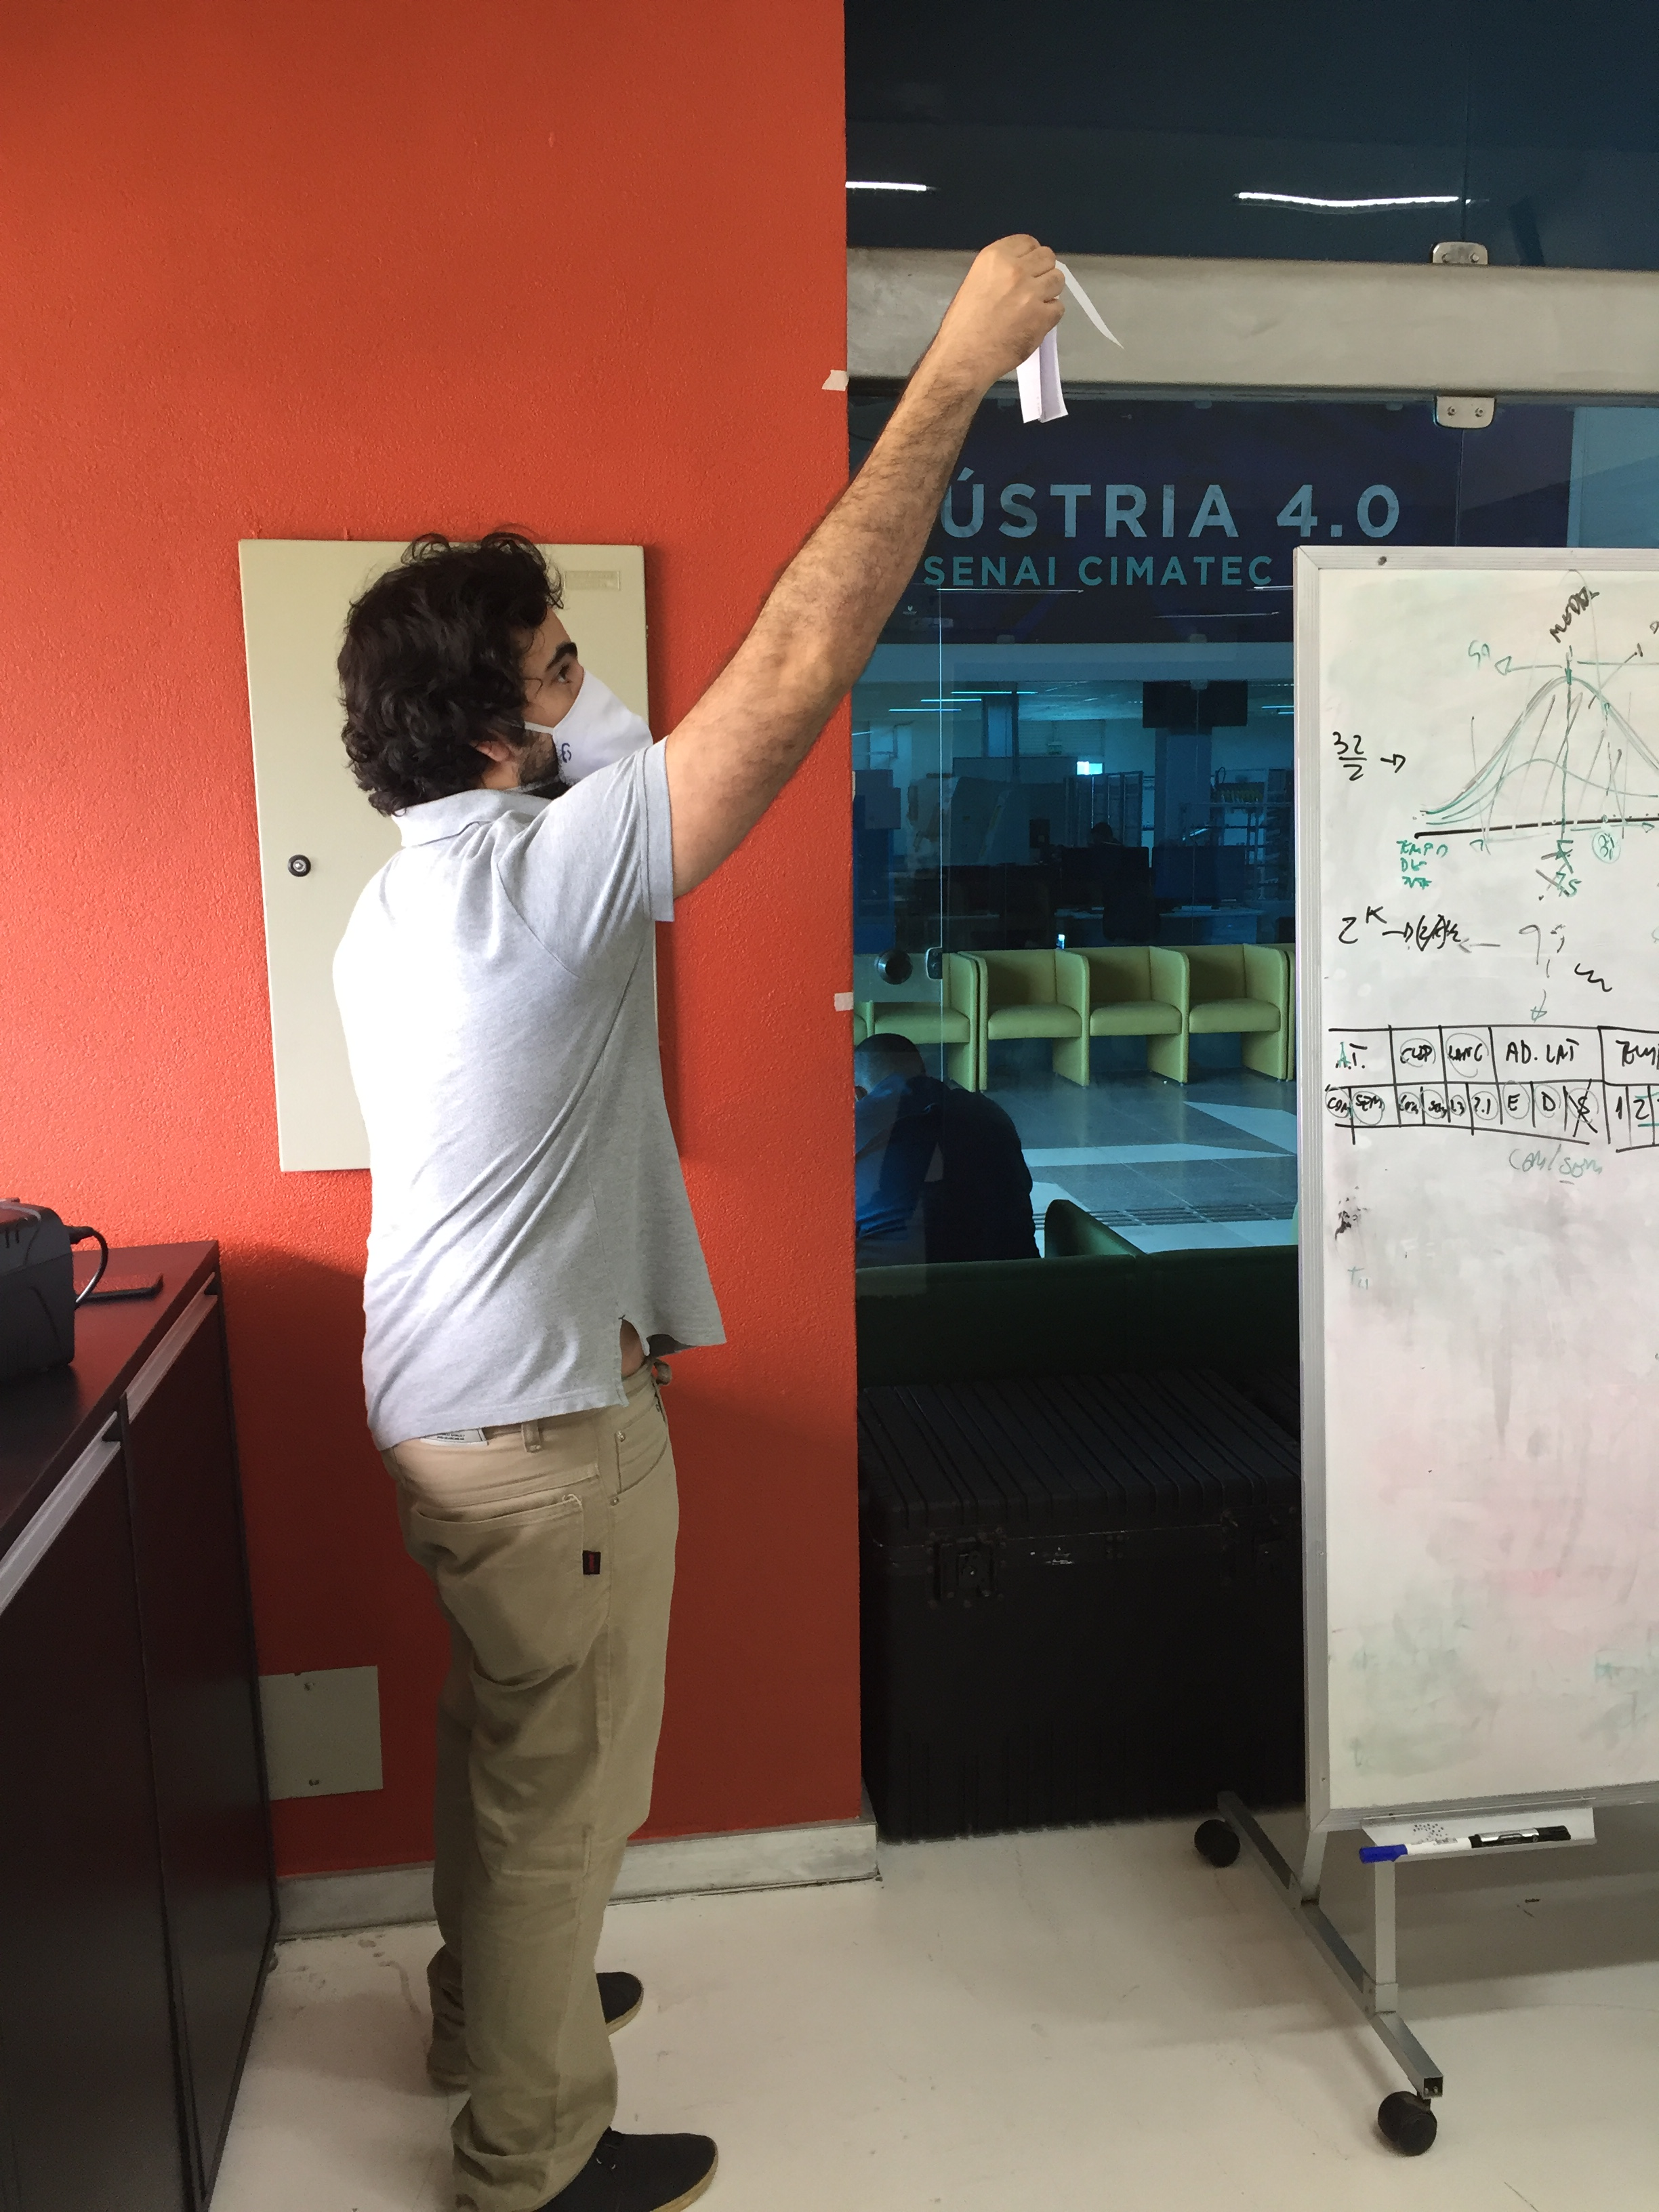
\includegraphics[width=0.4\textwidth]{images/20200909_145557439_iOS.png}\label{fig:f1}}
    \hfill
    \subfloat[1,3 metros.]{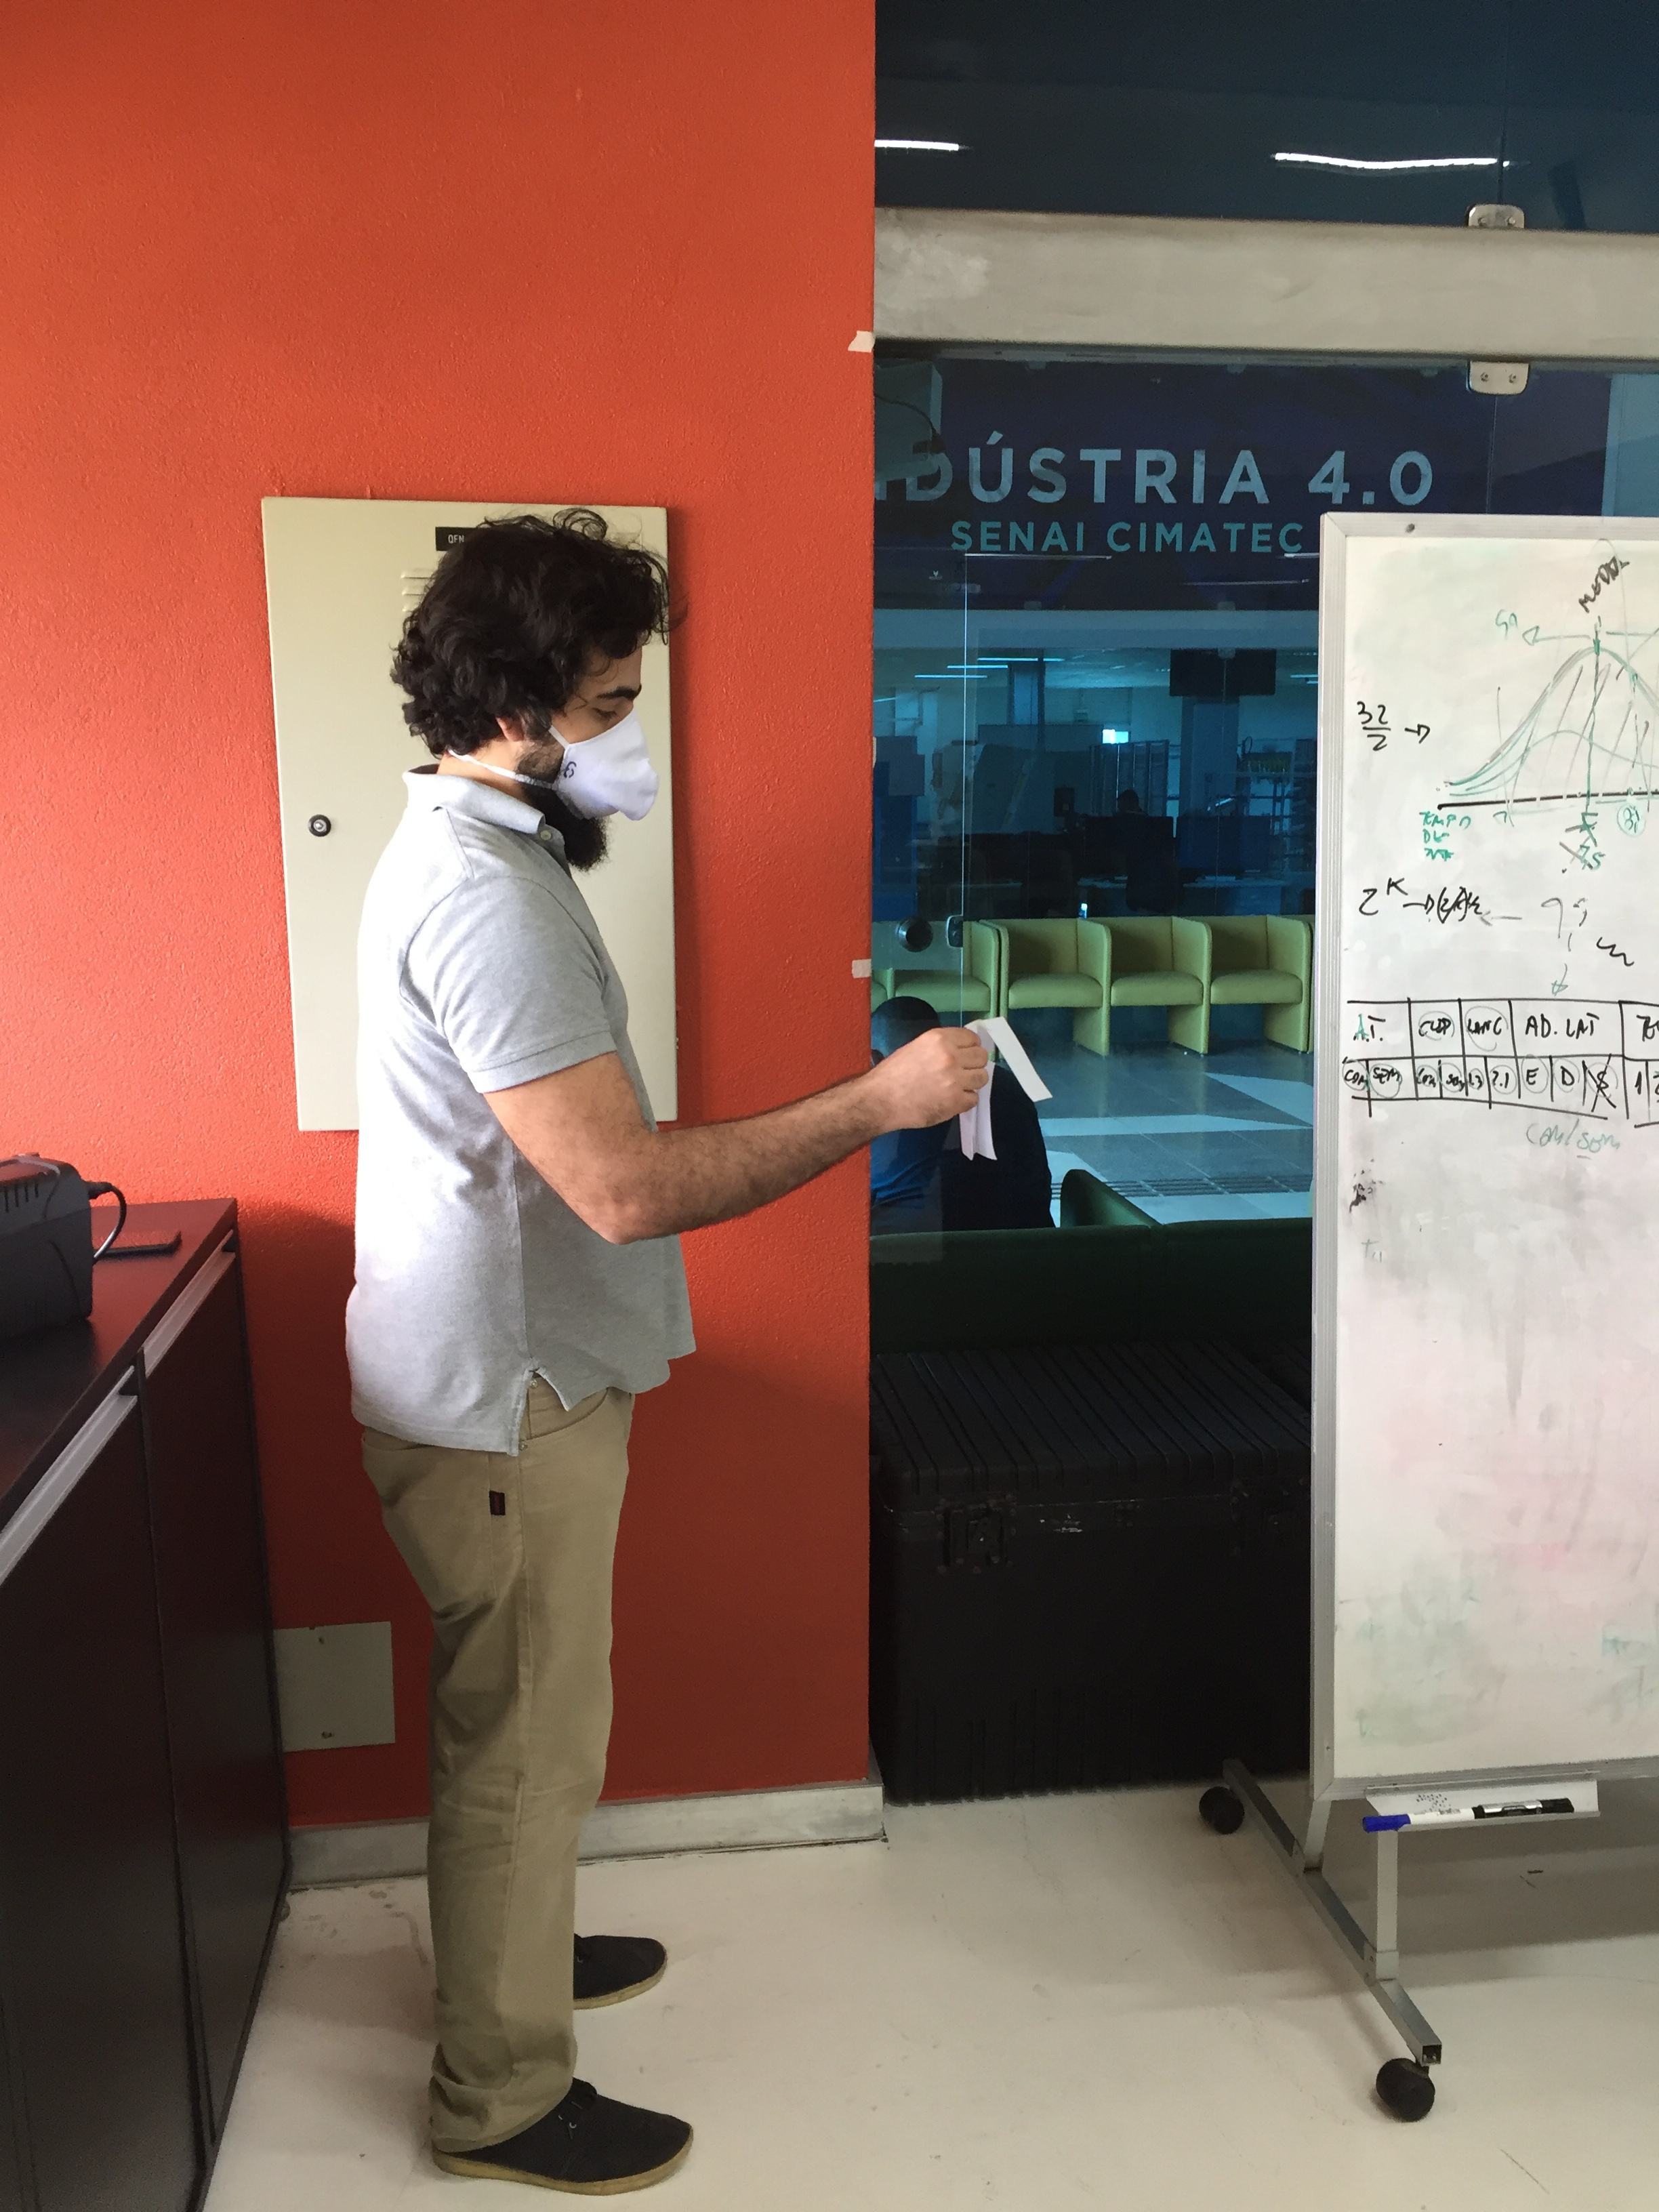
\includegraphics[width=0.4\textwidth]{images/20200909_145551403_iOS.png}\label{fig:f2}}
\caption{Altura de lançamento.}
  \end{figure}

  \begin{figure}[h]
    \centering
    \subfloat[Sem adições.]{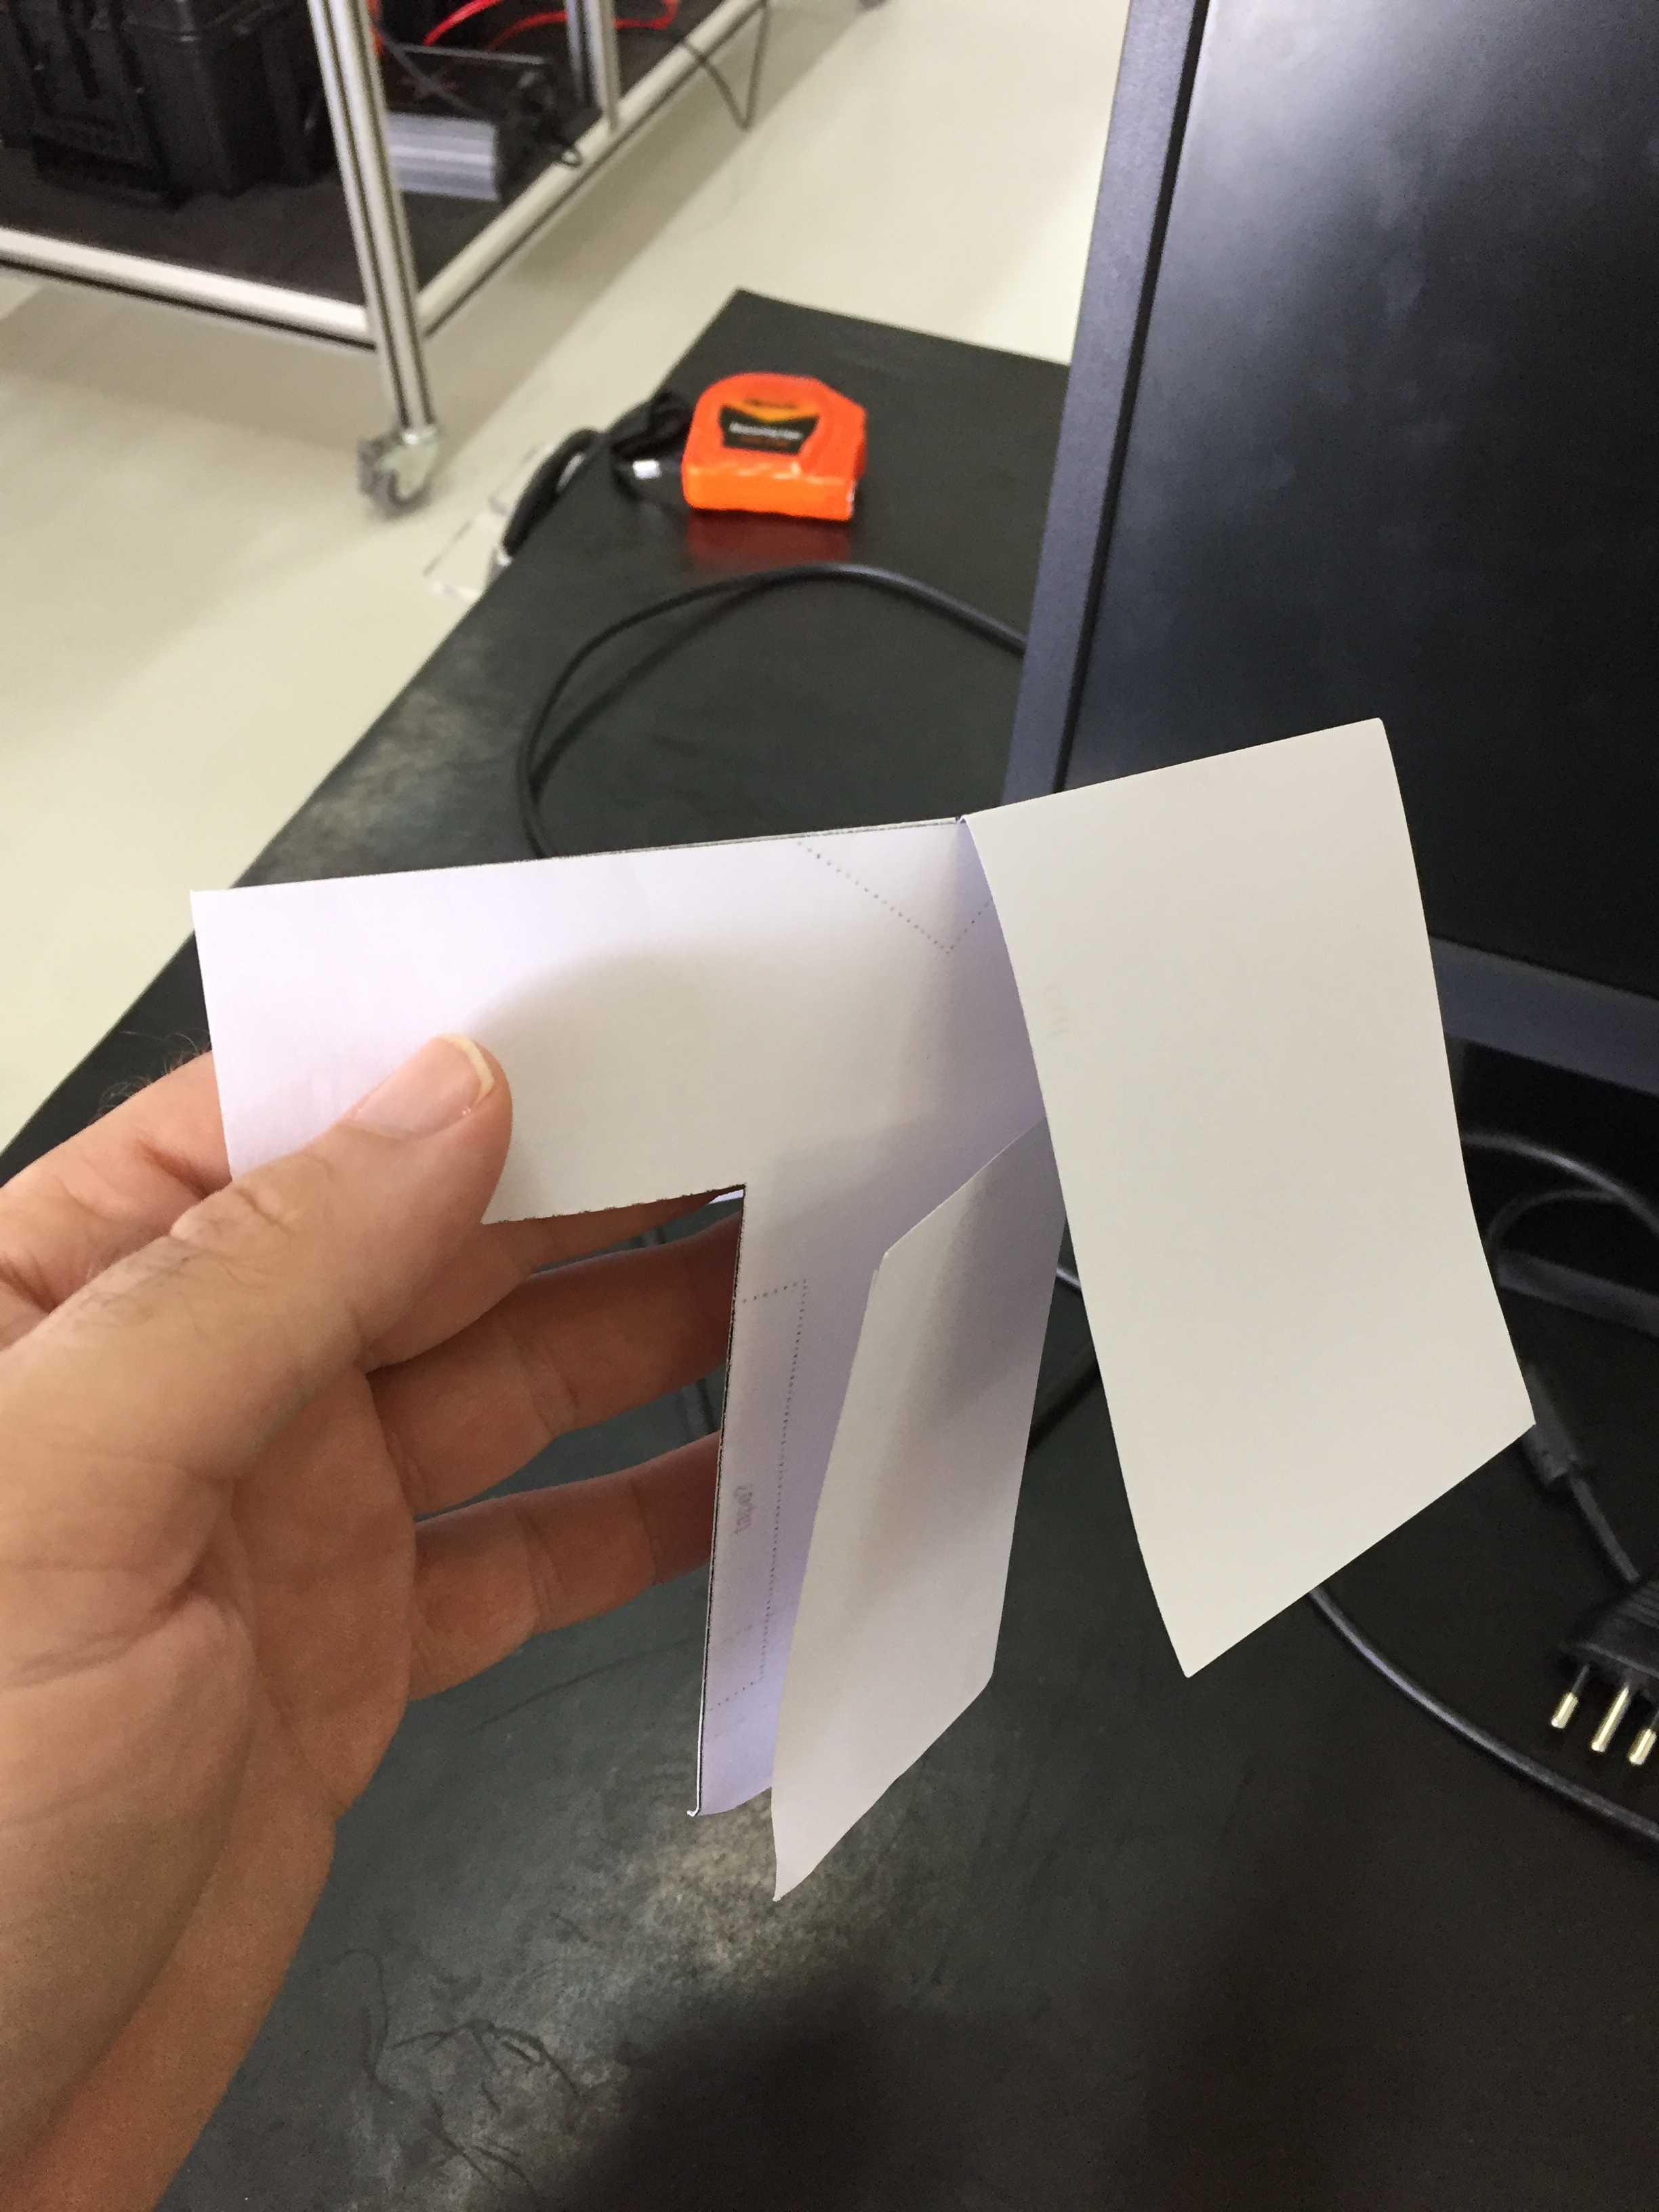
\includegraphics[width=0.4\textwidth]{images/sem_mudancas.png}\label{fig:f3}}
    \hfill
    \subfloat[Clipe na região inferior.]{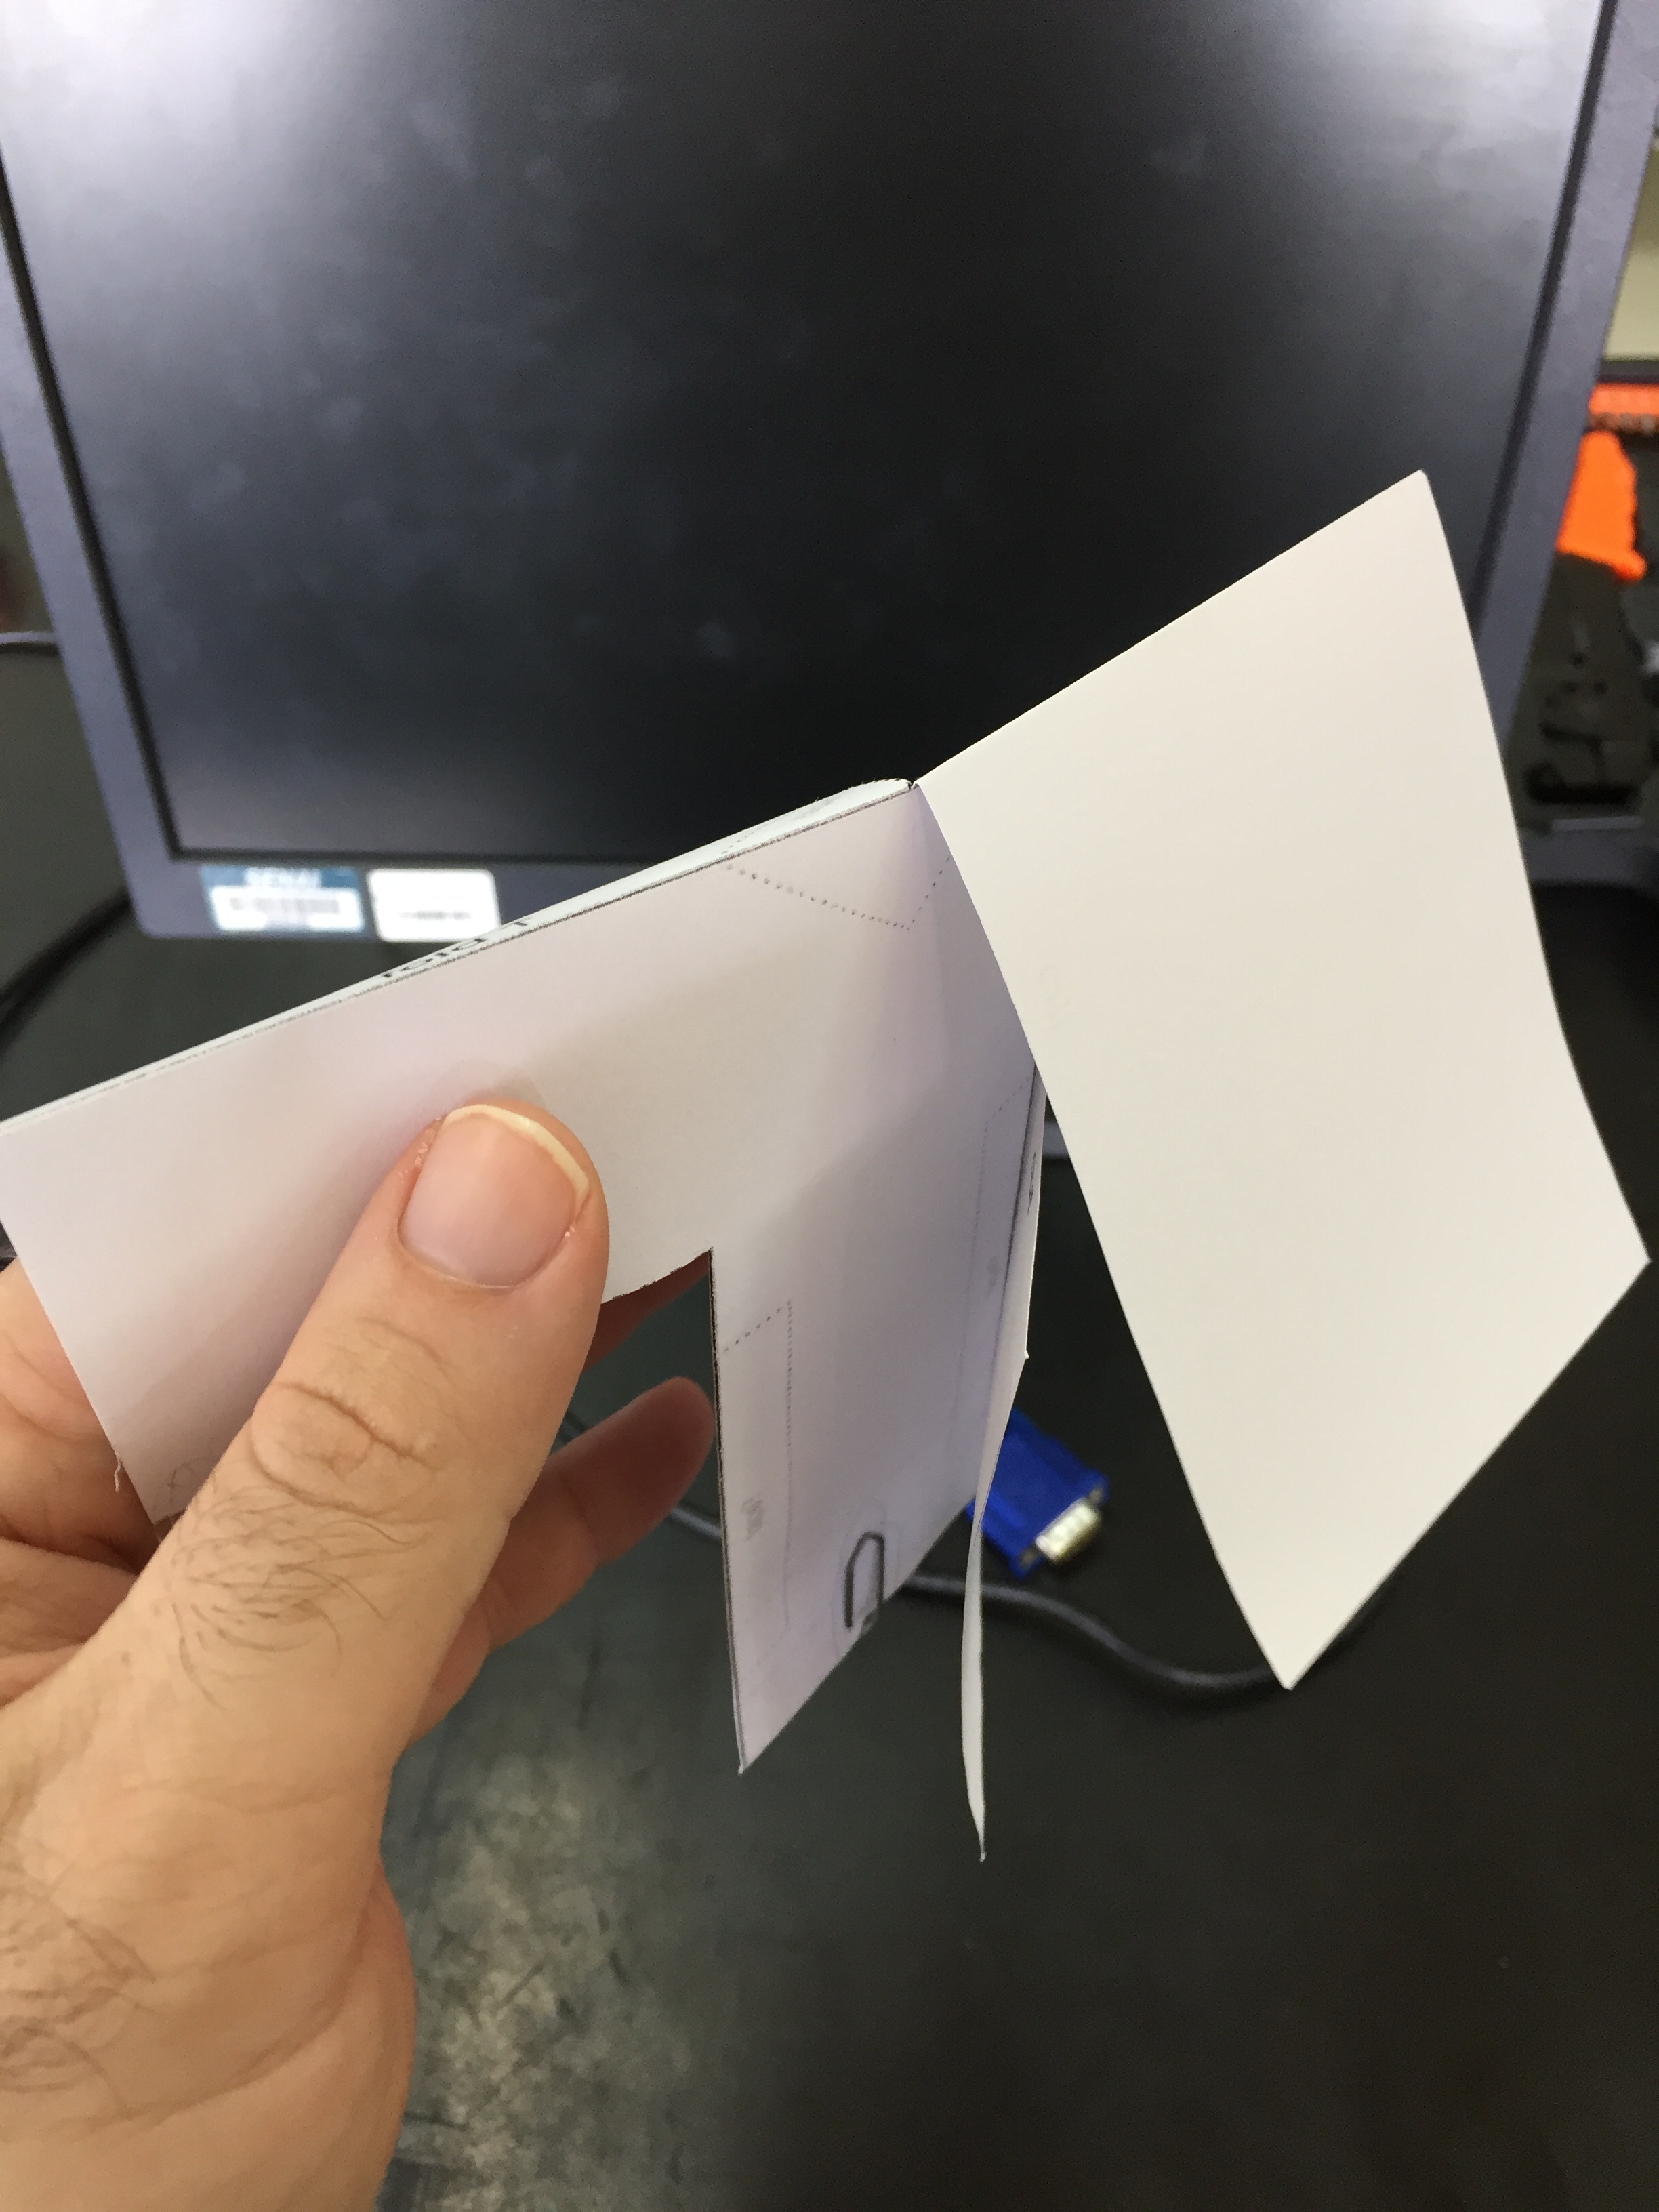
\includegraphics[width=0.4\textwidth]{images/clipe.png}\label{fig:f4}}
    \hfill
    \subfloat[Adesivo na lateral.]{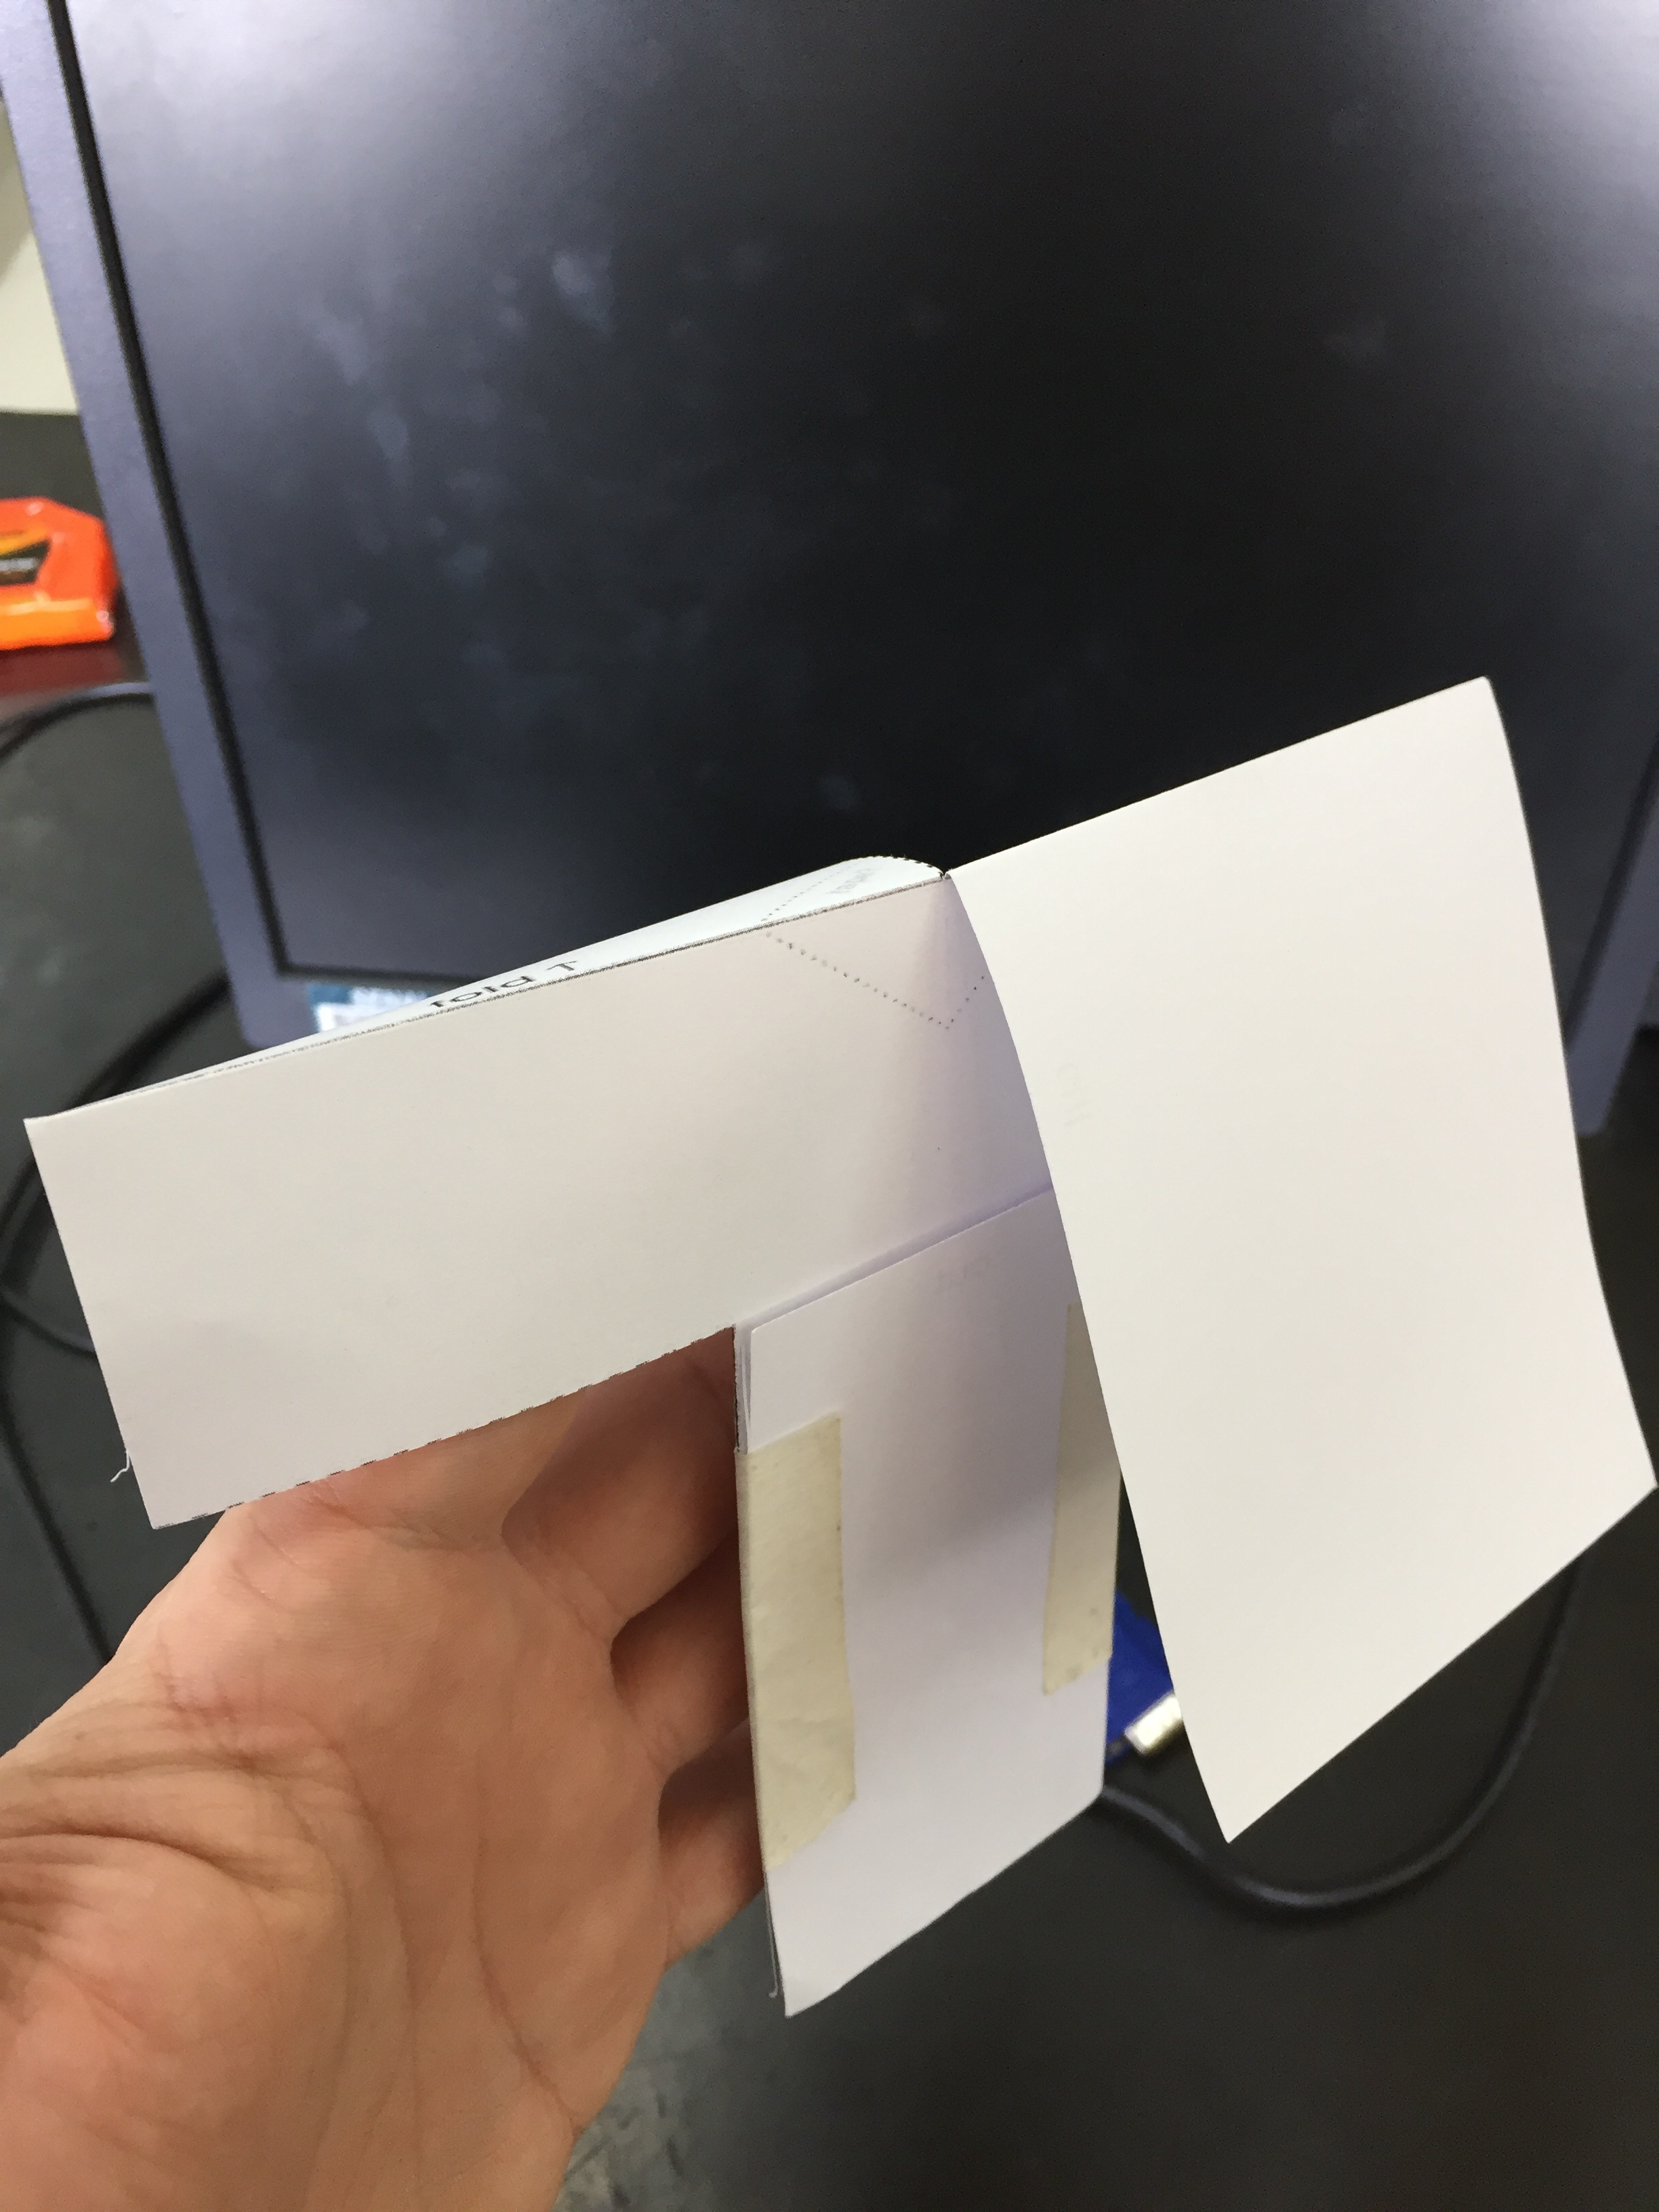
\includegraphics[width=0.4\textwidth]{images/adesivo_lateral.png}\label{fig:f5}}
    \hfill
    \subfloat[Adesivo no topo.]{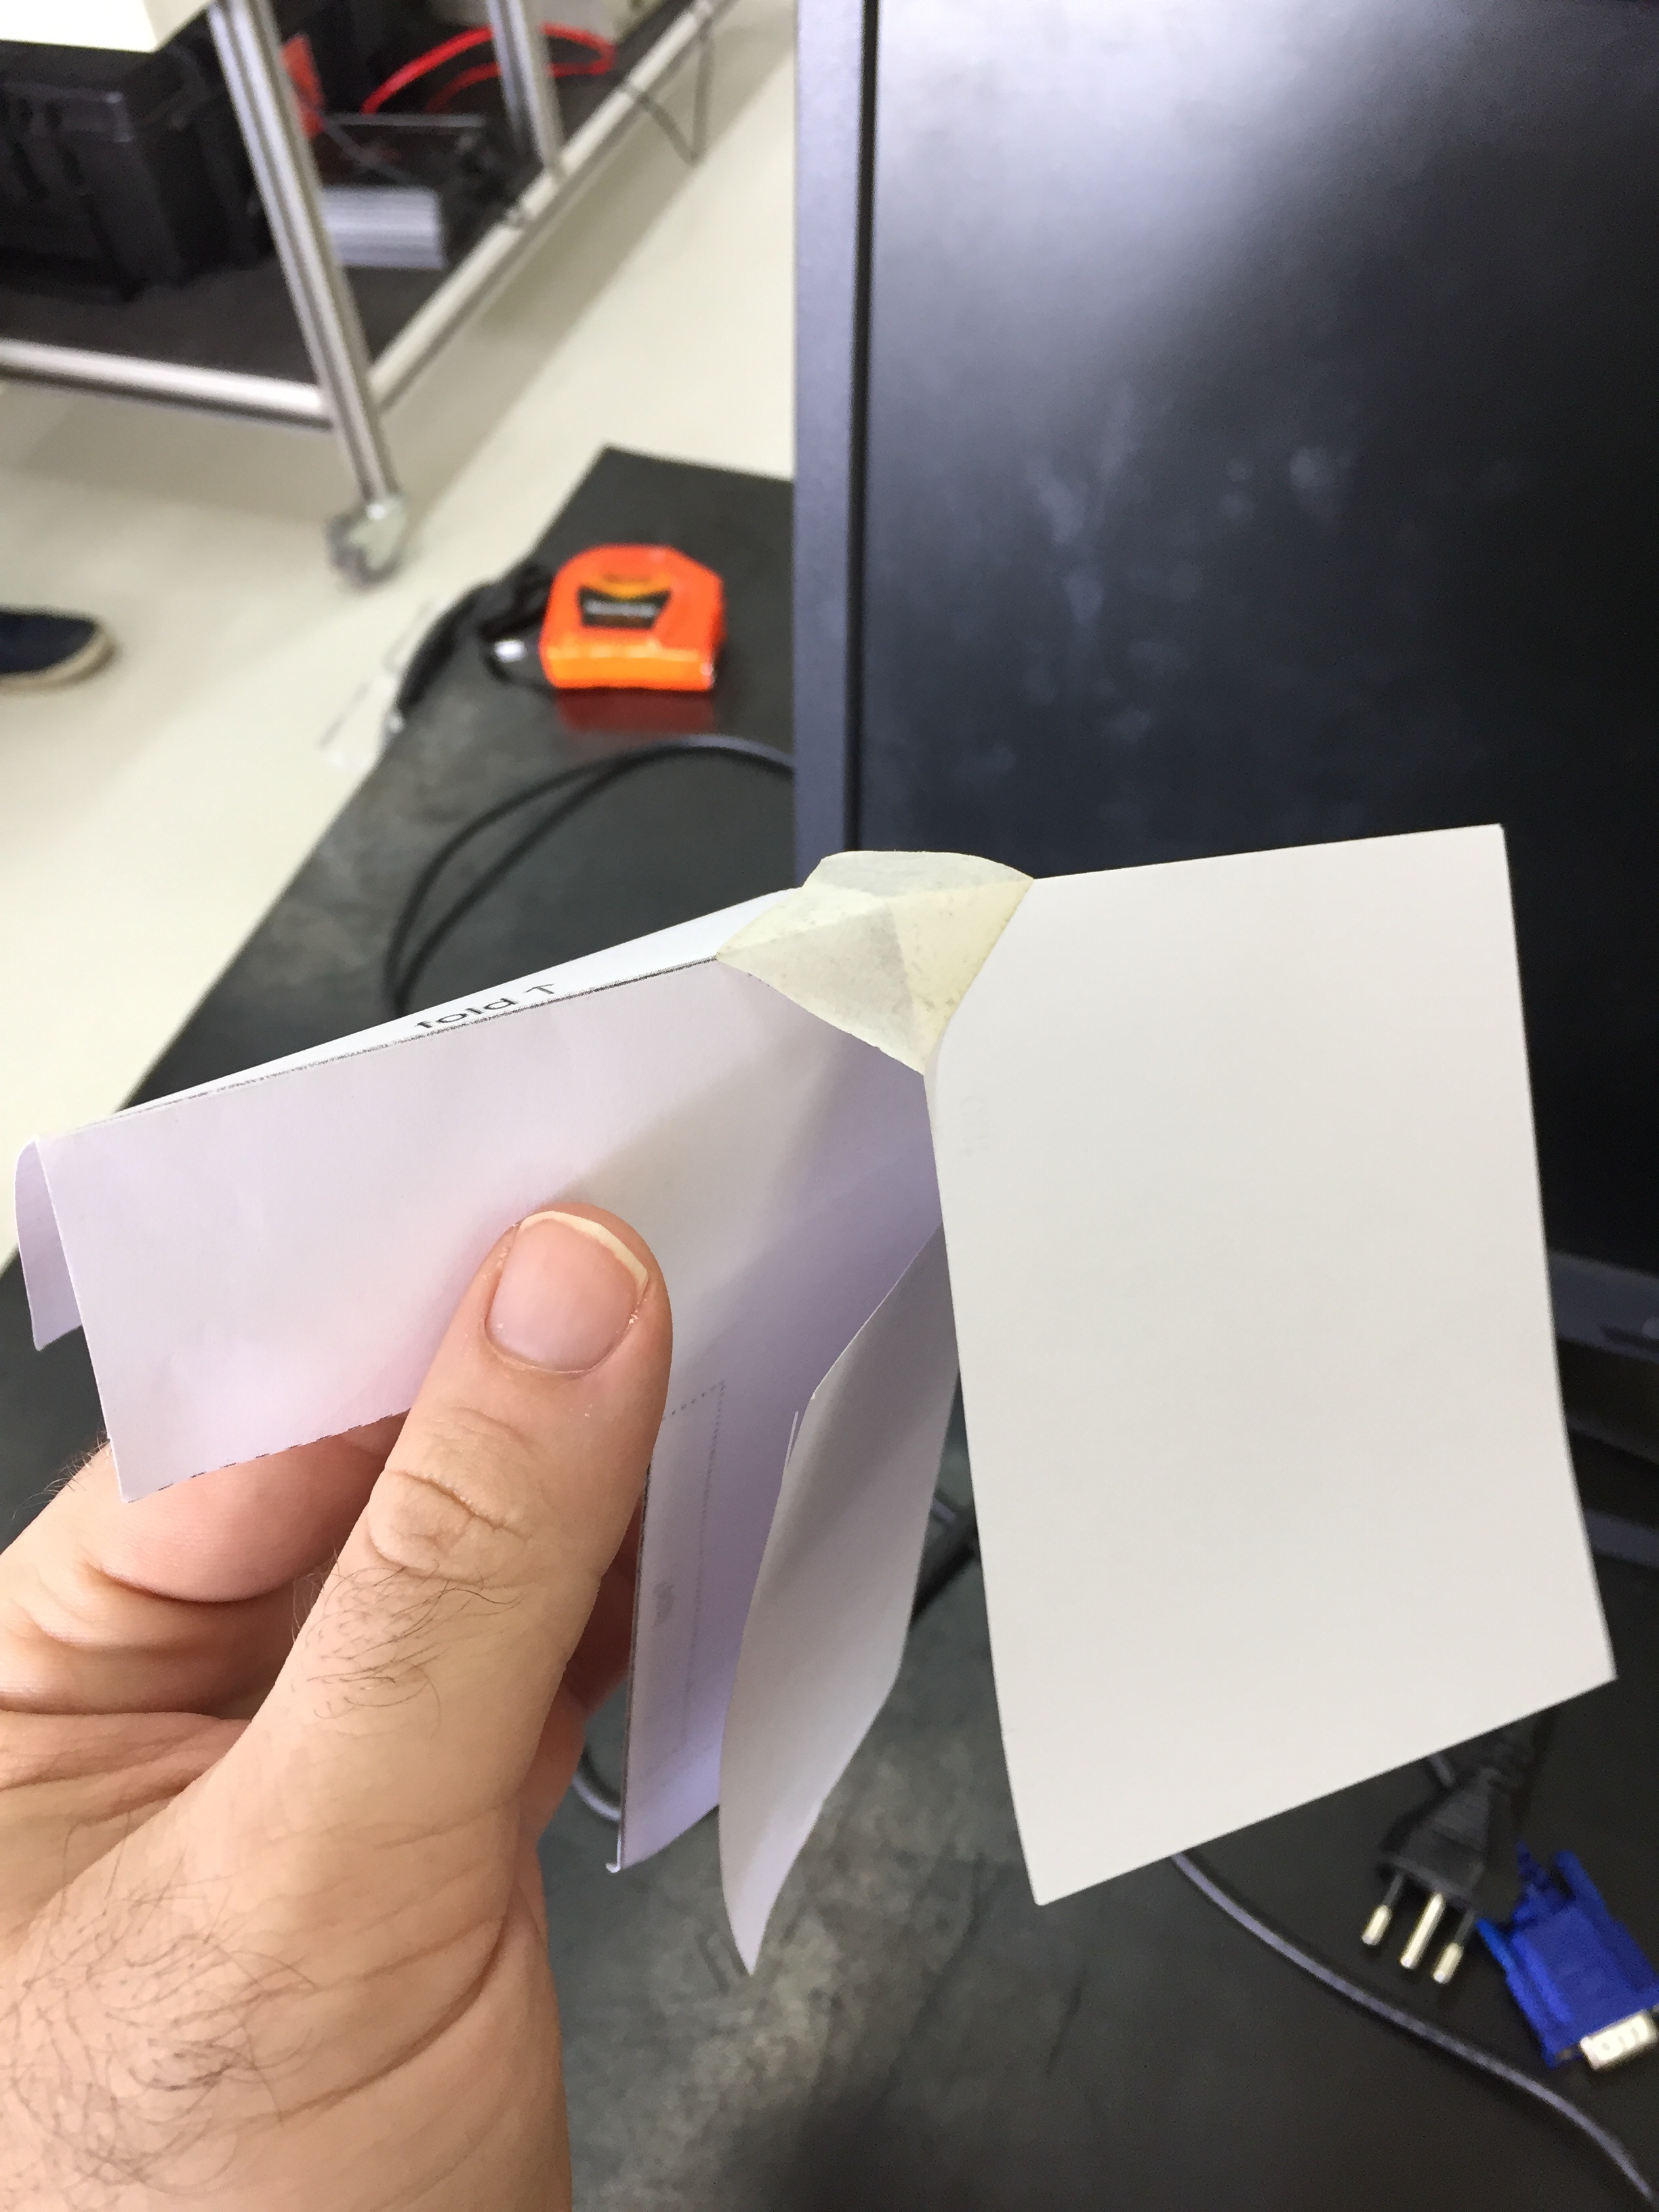
\includegraphics[width=0.4\textwidth]{images/adesivo_topo.png}\label{fig:f6}}
  \caption{Variações no corpo do helicóptero.}
  \end{figure}  

%! Escrever sobre as variáveis que foram testadas e as expectativas das suas influências -> se colocar o clipe, o peso aumenta e possivelmente o tempo de voo diminui etc...
	\chapter{Primeiro Experimento}
\label{chap:primeiro_experimento}

%! Escrever um pouco sobre o que foi feito

\section{Criando o experimento no R}
\label{sec:primeiro_experimento_criando o experimento_no_R}

%! Escrever sobre código usado para criar o experimento, a sequencia de testes, no R. Qual o motivo de usar isso?


\begin{table}[H]
  \centering
  \caption{Experimento de modelagem do helicóptero de papel.}
  \resizebox{0.7\textwidth}{!}{%
  \begin{tabular}{c|c|c|c}
  \textbf{Altura} & \textbf{Clipe} & \textbf{AdesivoTopo} & \textbf{AdesivoLateral} \\ \hline
  1.3             & -              & +                    & +                       \\ \hline
  2.1             & +              & +                    & -                       \\ \hline
  1.3             & -              & -                    & +                       \\ \hline
  2.1             & +              & -                    & -                       \\ \hline
  1.3             & +              & -                    & -                       \\ \hline
  2.1             & -              & +                    & -                       \\ \hline
  2.1             & -              & -                    & -                       \\ \hline
  1.3             & +              & +                    & +                       \\ \hline
  2.1             & -              & -                    & +                       \\ \hline
  1.3             & -              & -                    & -                       \\ \hline
  2.1             & +              & +                    & +                       \\ \hline
  2.1             & +              & -                    & +                       \\ \hline
  2.1             & -              & +                    & +                       \\ \hline
  1.3             & -              & +                    & -                       \\ \hline
  1.3             & +              & -                    & +                       \\ \hline
  1.3             & +              & +                    & -
  \end{tabular}%
  }
  \legend{Fonte: Autores.}
  \label{tab:experimento_modelagem_helicoptero_papel}
\end{table}

\section{A coleta de dados}
\label{sec:primeiro_experimento_a_coleta_de_dados}

%! Escrever sobre como foi feita a coleta de dados e indicar a tabela resultante
	\chapter{A Modelagem Matemática}
\label{chap:a_modelagem_matematica}

%! Escrever um pouco sobre o que foi feito

\section{Regressão linear}
\label{sec:a_modelagem_matematica_modelo_linear}

A Regressão Linear é utilizada para analisar as relações entre o valor de uma variável resultante Y e uma ou mais variáveis X e suas interações \cite{yang2020hyperparameter}. O objetivo desta técnica é obter um modelo matemático que seja capaz de representar um fenômeno, demonstrando mediante uma relação linear as relações entre a variável de entrada e a variável de saída. Vale destacar que após a criação do modelo, é possível estimar os valores da variável de resposta Y, utilizando valores conhecidos da variável preditora X.

A Regressão Linear modela uma variável $Y$ como uma função matemática de um ou mais variáveis $X$, e então esse modelo de regressão pode ser utilizado para obter $Y$ quando apenas o $X$ é conhecido. A função matemática genérica é dada pela Equação~\ref{eq1}:

\begin{equation}\label{eq1}
    Y = \beta_1 + \beta_2 * X + \epsilon
\end{equation}
%Y = B1 + B2X + E

% Figura

Onde o $\beta_1$ é a interceptação da reta com o eixo vertical e $\beta_2$ é a inclinação ou o coeficiente angular em relação à variável, eles são chamados de coeficientes de regressão \cite{medeiros2009aplicaccao}. O parâmetro $\epsilon$ é o erro, ou seja, a porção de $Y$ que o modelo de regressão não é capaz de explicar (Figura~\ref{fig:reg-lin}).

\begin{figure}[H]
    \centering
    \caption{Representação dos coeficientes do modelo linear.}
    \includegraphics[width=0.8\textwidth]{images/linear-regression.png}
    \legend{Fonte: \cite{reglin}.}
    \label{fig:reg-lin}
  \end{figure}

\section{Utilizando o modelo linear de primeira ordem}
\label{sec:a_modelagem_matematica_utilizando_o_modelo_linear}

O modelo utilizado é um modelo linear múltiplo de primeira ordem, para verificar o modelo matemático utilizando o código a seguir:

%! Colocar código

\lstinputlisting[language=R, firstline=41, lastline=43,inputencoding=latin1]{code/helicoptero_teste_media.R}

Neste modelo, são utilizados todos os parâmetros (Altura, Clipe, AdesivoTopo, AdesivoLateral), de modo a verificar quais variáveis tem maior interferência sobre o modelo final e então fazer um modelo linear levando em conta estas variáveis que mais representam este modelo. Os coeficientes obtidos utilizando o modelo linear são mostrados na Tabela~\ref{tab:primor}.

% Colocar figura ou tabela
% latex table generated in R 4.0.2 by xtable 1.8-4 package
% Mon Sep 21 19:24:02 2020
\begin{table}[h]
    \centering
    \caption{Modelo linear de primeira ordem.}
    \begin{tabular}{rrrrr}
      \hline
     & Estimate & Std. Error & t value & Pr($>$$|$t$|$) \\ 
      \hline
    (Intercept) & -0.1413 & 0.0763 & -1.85 & 0.0711 \\ 
      Altura & 0.8563 & 0.0406 & 21.08 & 0.0000 \\ 
      Clipe+ & -0.1100 & 0.0325 & -3.38 & 0.0015 \\ 
      AdesivoTopo+ & 0.0592 & 0.0325 & 1.82 & 0.0757 \\ 
      AdesivoLateral+ & 0.0300 & 0.0325 & 0.92 & 0.3611 \\ 
       \hline
    \end{tabular}
    \label{tab:primor}
    \end{table}



O valor $\beta_1$, correspondente à interceptação da reta é mostrado na primeira linha. Os valores corespondentes à inclinação ($\beta_2$) são mostrados na coluna "Estimate", visto que estes são os valores correspondentes a cada variável. Logo, o modelo pode ser medido pela seguinte equação:

\begin{equation}\label{eq2}
Y = - 0.14125 + 0.85625 * Altura - 0.11 * Clipe + 0.05917 * AdesivoTopo + 0.03 * AdesivoLateral
\end{equation}

Na Equação~\ref{eq2}, a modelagem do helicóptero é dada em função da altura, da presença do clipe e dos adesivos, tanto no topo quanto na lateral. Um aspecto que também deve ser levado em consideração é o p-valor dos coeficientes do modelo linear. O p-valor indica a hipótese deve ser rejeitada ou aceita, neste caso, a hipótese é que o preditor não é significativo para o modelo. Nesta avaliação, para verificar se os preditores são significativos ou não, é verificar se os valores de $p$ são menores que 0,05.

Na análise do modelo, existem dois p-valores de dois preditores que são muito abaixo de 0.05, que são Altura e Clipe. Estes pequenos valores indicam que provavelmente Altura e Clipe sejam uma ótima adição ao modelo. Os valores de p-valor para as variáveis AdesivoTopo e Adesivo lateral são 0.076 e 0.36, respectivamente. Esses valores indicam que existe aproximadamente 8\% e 36\% de chances que essas variáveis não sejam significativas para a regressão, respectivamente.

\subsection{Residuos}

Para testar a qualidade do ajuste do modelo, um parâmetro considerado é a observação dos resíduos, que são as diferenças entre os valores reais e os valores preditos \cite{schneider2010linear}. Como a regressão linear é o processo de traçar uma reta através dos dados em um diagrama de dispersão, a reta principal representa os valores preditos. Os resíduos são a mínima distância entre os valores preditos e os valores reais, representados pelas retas vermelhas na Figura~\ref{fig:residuos}. 

% Colocar figura

\begin{figure}[H]
    \centering
    \caption{Representação dos resíduos do modelo linear.}
    \includegraphics[width=0.5\textwidth]{images/residuos.png}
    \legend{Fonte: \cite{reglin}.}
    \label{fig:residuos}
  \end{figure}

O ideal seria que os valores de resíduos atingissem um valor igual ou próximo de zero, entretanto em aplicaçõas reais pode ser que esses valores de resíduos não sejam atingidos. No modelo testado, os valores obtidos estão situados em uma faixa entre -0.36 e 0.3, e a mádia de todos os valores atinge um valor de 0.00104, valor este muito próximo de zero.

Os gráficos gerados utilizando este modelo mostrando os residuais estão representados na Figura~\ref{fig:residuos-plot}.

\begin{figure}[H]
    \centering
    \caption{Gráficos dos resíduos do modelo linear.}
    \includegraphics[width=0.8\textwidth]{images/model1ordem.png}
    \legend{Fonte: Autores.}
    \label{fig:residuos-plot}
  \end{figure}

\subsection{Múltiplo R-quadrado}

Para testar a qualidade do modelo gerado é utilizada a medida do coeficiente de determinação, ou simplesmente $R^2$, que é medido através da proporção da variabilidade total explicada pelo modelo de regressão. Para modelos que se ajustam bem aos dados, $R^2$ é próximo a 1, e modelos que se ajustam mal aos dados têm $R^2$ próximo de 0 \cite{schneider2010linear}. No modelo gerado, foi obtido um valor de $R^2$ múltiplo de 0.9145, ou seja, o modelo pode explicar 91.45\% da variabilidade total.

O modelo entrega dois valores de $R^2$ diferentes, um múltiplo e um ajustado. Uma desvantagen do $R^2$ múltiplo é que ele continuará aumentando à medida o modelo se torna mais complexo, mesmo que essas variáveis ​​não adicionem nada às previsões. O $R^2$ ajustado é uma melhor métrica caso exista mais de uma variável no modelo, uma vez que ele só cresce se erro geral das predições for reduzido. Neste caso, o valor obtido do $R^2$ ajustado é 0.9065. 


% Colocar formula







%! Escrever sobre código usado para criar o modelo linear, como este é capaz de utilizar não linearidades

\section{Utilizando o modelo linear de segunda ordem}
\label{sec:a_modelagem_matematica_o_modelo_resultante}

%! Escrever sobre o resultado encontrado e o que ele nos informa

Em seguida foi utilizado um modelo linear múltiplo de segunda ordem, para verificar se haveria alguma interação de segunda ordem significativa, além daquelas encontradas nas variáveis "Altura" e "Clipe". O modelo matemático utilizando o código a seguir:

%! Colocar código

\lstinputlisting[language=R, firstline=50, lastline=52,inputencoding=latin1]{code/helicoptero_teste_media.R}

Neste modelo, também são utilizados todos os parâmetros (Altura, Clipe, AdesivoTopo, AdesivoLateral), e as suas interações de segunda ordem. Os coeficientes obtidos utilizando o modelo linear são mostrados na Tabela~\ref{tab:segor}.

% latex table generated in R 4.0.2 by xtable 1.8-4 package
% Mon Sep 21 20:56:39 2020
\begin{table}[ht]
    \centering
    \caption{Modelo linear de segunda ordem.}
    \begin{tabular}{rrrrr}
      \hline
     & Estimate & Std. Error & t value & Pr($>$$|$t$|$) \\ 
      \hline
    (Intercept) & 0.0341 & 0.1455 & 0.23 & 0.8159 \\ 
      Altura & 0.7464 & 0.0817 & 9.14 & 0.0000 \\ 
      Clipe+ & -0.3476 & 0.1500 & -2.32 & 0.0261 \\ 
      AdesivoTopo+ & 0.0028 & 0.1500 & 0.02 & 0.9851 \\ 
      AdesivoLateral+ & -0.0039 & 0.1500 & -0.03 & 0.9796 \\ 
      Altura:Clipe+ & 0.1260 & 0.0817 & 1.54 & 0.1314 \\ 
      Altura:AdesivoTopo+ & 0.0469 & 0.0817 & 0.57 & 0.5696 \\ 
      Altura:AdesivoLateral+ & 0.0469 & 0.0817 & 0.57 & 0.5696 \\ 
      Clipe+:AdesivoTopo+ & 0.0458 & 0.0654 & 0.70 & 0.4875 \\ 
      Clipe+:AdesivoLateral+ & 0.0008 & 0.0654 & 0.01 & 0.9899 \\ 
      AdesivoTopo+:AdesivoLateral+ & -0.0925 & 0.0654 & -1.42 & 0.1654 \\ 
       \hline
    \end{tabular}
    \label{tab:segor}
    \end{table}

A modelagem do helicóptero é dada em função da altura, da presença do clipe e dos adesivos, tanto no topo quanto na lateral e ainda nas interações entre estas variáveis. Na análise do modelo, também existem dois p-valores de dois preditores que são muito abaixo de 0.05, que são $Altura$ e $Clipe$. O p-valor das variáveis $Altura$ e $Clipe$ são $5.08e^(-11)$ e $0.0261$, respectivamente. Os valores de p-valor para as demais variáveis e suas interações ultrapassam o valor de 0.05, logo, não são significativas para a regressão.

\subsection{Residuos}

No modelo testado, os valores obtidos estão situados em uma faixa entre -0.30146 e 0.29396, e a mádia de todos os valores atinge um valor de 0.01646, valor este muito próximo de zero.

Os gráficos gerados utilizando este modelo mostrando os residuais estão representados na Figura~\ref{fig:residuos-plot2}.

\begin{figure}[H]
    \centering
    \caption{Gráficos dos resíduos do modelo linear.}
    \includegraphics[width=0.8\textwidth]{images/model2ordem.png}
    \legend{Fonte: Autores.}
    \label{fig:residuos-plot2}
  \end{figure}


  \subsection{Múltiplo R-quadrado}

No modelo gerado, foi obtido um valor de $R^2$ múltiplo de 0.9256, ou seja, o modelo pode explicar 92.56\% da variabilidade total, e o valor obtido do $R^2$ ajustado é 0.9055. 

Nesta abordagem, concluiu-se que não houve uma significativa diferença entre o modelo de primeira ordem e o modelo de segunda ordem. Na comparação entre os dois modelos verificou-se que somente as variáveis "Altura" e "Clipe" eram significativas para explicar o modelo. Logo, pode-se concluir que o modelo de primeira ordem é suficiente para representar o helicóptero.
	\chapter{Segundo Experimento}
\label{chap:segundo_experimento}

%! Escrever um pouco sobre o que foi feito

Analogamente aos experimentos realizados no Capítulo \ref{chap:primeiro_experimento}, foi gerado um conjunto de experimentos com o intuito de verificar o modelo matemático proposto no Capítulo \ref{chap:a_modelagem_matematica}. Os novos experimentos buscam então avaliar o modelo linear proposto com base apenas nas variáveis altura do lançamento e presença do clipe no helicóptero de papel.

\section{Criando o experimento no R}
\label{sec:segundo_experimento_criando o experimento_no_R}

%! Escrever sobre código usado para criar o experimento, a sequencia de testes, no R. Qual o motivo de usar isso?

O código originalmente criado para a formulação do primeiro conjunto de experimentos, disposto no Apêndice \ref{sec:app_codigo_geracao_do_experimento_de_modelagem}, foi modificado de forma a gerar o novo conjunto de experimentos, Apêndice \ref{sec:app_codigo_geracao_do_experimento_para_teste_do_modelo}. A sequência de variações dos parâmetros do helicóptero de papel a serem realizadas neste experimento está disposta na Tabela \ref{tab:experimentos_para_teste_do_modelo}.

\begin{table}[H]
  \centering
  \caption{Experimentos para teste do modelo.}
  \resizebox{0.25\textwidth}{!}{%
  \begin{tabular}{c|c}
  \textbf{Altura} & \textbf{Clipe} \\ \hline
  1.7             & -              \\ \hline
  1.7             & +              \\ \hline
  1.0             & -              \\ \hline
  1.0             & +              \\ \hline
  2.2             & +              \\ \hline
  1.5             & +              \\ \hline
  1.5             & -              \\ \hline
  2.2             & -
  \end{tabular}%
  }
  \legend{Fonte: Autores.}
  \label{tab:experimentos_para_teste_do_modelo}
\end{table}

\section{A coleta de dados}
\label{sec:segundo_experimento_a_coleta_de_dados}

Os dados coletados estão dispostos na Tabela \ref{tab:dados_experimentais_teste_modelo}. A coleta destes dados seguiu o mesmo procedimento do Experimento 1, apresentado na Seção \ref{sec:primeiro_experimento_a_coleta_de_dados}.

%! Escrever sobre como foi feita a coleta de dados e indicar a tabela resultante
	\chapter{Verificação do Modelo}
\label{chap:verificacao_do_modelo}

%! Escrever um pouco sobre o que foi feito
Após a comprovação de que as variáveis $Clipe$ e $Altura$ são as mais significativas na criação do primeiro modelo, foi criado um modelo linear de primeira ordem contemplando somente estas duas variávei, utilizando os dados medidos para teste. Os coeficientes obtidos utilizando o modelo linear são mostrados na Tabela~\ref{tab:terc-mod}.

% latex table generated in R 4.0.2 by xtable 1.8-4 package
% Mon Sep 21 23:47:47 2020
\begin{table}[ht]
    \centering
    \caption{Modelo linear de primeira ordem.}
    \begin{tabular}{rrrrr}
      \hline
     & Estimate & Std. Error & t value & Pr($>$$|$t$|$) \\ 
      \hline
    (Intercept) & -0.0967 & 0.0745 & -1.30 & 0.2012 \\ 
      Altura & 0.8563 & 0.0416 & 20.59 & 0.0000 \\ 
      Clipe+ & -0.1100 & 0.0333 & -3.31 & 0.0019 \\ 
       \hline
    \end{tabular}
    \label{tab:terc-mod}
    \end{table}

No modelo testado, os valores obtidos estão situados em uma faixa entre -0.40146 e 0.28854, e a mádia de todos os valores atinge um valor de 0.00354. Os gráficos gerados utilizando este modelo mostrando os residuais estão representados na Figura~\ref{fig:residuos-plot3}.

\begin{figure}[H]
    \centering
    \caption{Gráficos dos resíduos do modelo linear.}
    \includegraphics[width=0.8\textwidth]{images/model.png}
    \legend{Fonte: Autores.}
    \label{fig:residuos-plot3}
  \end{figure}

  No modelo gerado, foi obtido um valor de $R^2$ múltiplo de 0.9062, ou seja, o modelo pode explicar 90.62\% da variabilidade total, e o valor obtido do $R^2$ ajustado é 0.902. 

\section{Utilizando a correlação de dados}
\label{sec:verificacao_do_modelo_utilizando_a_correlacao_de_dados}

%! Escrever sobre código usado para correlacionar os dados preditos com os encontrados no segundo experimento

Em seguida, foram utilizados como dados de entrada as alturas utilizadas no segundo experimento, e em seguida submetidas ao modelo gerado no primeiro experimento. Em seguida, os resultados obtidos com esta predição foram comparadas aos dados empíricos obtidos no segundo experimento, utilizando a correlação de Pearson. 

\section{O resultado}
\label{sec:verificacao_do_modelo_o_resultado}

%! Escrever sobre o resultado encontrado e o que ele nos informa

O resultado encontrado indica que o modelo gerado no experimento foi capaz de obter uma correlação de 0.9880744 com os testes empíricos. Estes experimentos significam que o modelo gerado foi capaz de descrever o helicóptero com um modelo matemático que se assemelha bastante aos resultados reais, obtidos em teste. Os gráficos gerados da correlação, comparando as predições feitas no primeiro modelo com os resultados dos testes estão representados na Figura~\ref{fig:corr}.

\begin{figure}[H]
    \centering
    \caption{Gráficos da correlação entre o modelo gerado e testes empíricos.}
    \includegraphics[width=0.8\textwidth]{images/corr.png}
    \legend{Fonte: Autores.}
    \label{fig:corr}
  \end{figure}
	\chapter{CONCLUSÃO}
\label{chap:conclusao}

Este trabalho apresentou os resultados do experimento de modelagem matemática de um helicóptero de papel. Com base na teoria de \ac{DOE}, foram escolhidas possíveis alterações no modelo físico do helicóptero de forma a investigar o efeito destas alterações no tempo de vôo do helicóptero. As quatro variáveis investigadas foram a altura de lançamento, a presença de clipe de papel na sua base, de adesivo no topo conectando as duas hélices e de adesivo em ambos os lados do corpo.

Através da análise realizada, foi possível gerar um modelo linear relacionando o tempo de vôo com a altura de lançamento e com a presença do clipe de papel, sendo a primeira diretamente proporcional e a segunda inversamente proporcional. Logo, o modelo indica que quanto mais elevado for o ponto de partida, maior será o tempo de vôo, por outro lado a presença do clipe de papel diminui o tempo de vôo. Tais resultados estão de acordo com o esperado, uma vez que a elevação da altura aumenta a distância a ser percorrida e a presença do clipe aumenta a massa do helicóptero.

Além do modelo matemático encontrado estar condizente com o esperado, os resultados da análise de correlação entre os valores preditos pelo modelo e os encontrados no experimento definido no Capítulo \ref{chap:segundo_experimento}, tal como visto no Capítulo \ref{chap:verificacao_do_modelo}, foram excelentes com valor de correlação de 99\%. Estes resultados evidenciam a aplicabilidade da teoria de \ac{DOE} e de modelagem matemática através da aplicação das técnicas de aproximação linear com fatores possivelmente não lineares.

% --------------------------------------------------------------------------
% Referências
	% \cleardoublepage
	\titleformat{\chapter}[display]{\vspace*{-24pt}\ABNTEXchapterfont\large\bfseries}{\chaptertitlename\ \thechapter}{12pt}{\Large}
	\bibliography{bibliography}
% --------------------------------------------------------------------------
% Apêndices
\apendices
\justify
\chapter{Tabelas de dados dos experimentos}
\label{chap:app_tabelas_de_dados_dos_experimentos}

Os dados experimentais encontrados para o tempo de vôo do modelo de helicóptero de papel estão apresentados a seguir. A Seção \ref{sec:app_experimento_1} - Experimento 1 apresenta os resultados obtidos a partir dos experimentos gerados na Seção \ref{sec:primeiro_experimento_criando o experimento_no_R} e apresentados na Tabela \ref{tab:experimento_modelagem_helicoptero_papel}. Analogamente, a Seção \ref{sec:app_experimento_2} - Experimento 2 apresenta os dados encontrados para o experimento da Seção \ref{sec:segundo_experimento_criando o experimento_no_R} e apresentados na Tabela \ref{tab:experimentos_para_teste_do_modelo}.

\section{Experimento 1}
\label{sec:app_experimento_1}

\begin{table}[H]
  \caption{Dados experimentais para modelagem.}
  \resizebox{\textwidth}{!}{%
  \begin{tabular}{c|c|c|c|c|c}
  \textbf{Teste1\_Mateus} & \textbf{Teste1\_Pedro} & \textbf{Teste2\_Mateus} & \textbf{Teste2\_Pedro} & \textbf{Teste3\_Mateus} & \textbf{Teste3\_Pedro} \\ \hline
  0.90 & 1.05 & 0.73 & 1.03 & 1.12 & 0.98 \\ \hline
  1.61 & 1.61 & 1.71 & 1.73 & 1.59 & 1.79 \\ \hline
  1.22 & 1.14 & 1.18 & 1.05 & 1.02 & 0.93 \\ \hline
  1.61 & 1.47 & 1.52 & 1.59 & 1.54 & 1.55 \\ \hline
  0.86 & 0.93 & 0.84 & 0.76 & 0.88 & 0.92 \\ \hline
  1.60 & 1.67 & 1.78 & 1.66 & 1.82 & 1.85 \\ \hline
  1.70 & 1.71 & 1.35 & 1.25 & 1.56 & 1.66 \\ \hline
  0.95 & 0.98 & 1.13 & 0.92 & 0.94 & 1.05 \\ \hline
  1.98 & 2.00 & 1.75 & 1.63 & 1.52 & 1.56 \\ \hline
  1.02 & 1.02 & 1.04 & 1.02 & 0.96 & 0.91 \\ \hline
  1.47 & 1.66 & 1.63 & 1.62 & 1.82 & 1.65 \\ \hline
  1.55 & 1.45 & 1.60 & 1.72 & 1.71 & 1.60 \\ \hline
  1.69 & 1.74 & 1.79 & 1.83 & 1.53 & 1.60 \\ \hline
  1.15 & 1.14 & 0.94 & 1.10 & 1.20 & 1.15 \\ \hline
  0.82 & 0.92 & 0.83 & 0.80 & 0.76 & 0.76 \\ \hline
  0.93 & 0.73 & 0.79 & 0.81 & 0.92 & 0.92
  \end{tabular}%
  }
  \legend{Fonte: Autores.}
  \label{tab:dados_experimentais_para_modelagem}
\end{table}

\section{Experimento 2}
\label{sec:app_experimento_2}

\begin{table}[H]
  \caption{Dados experimentais para teste do modelo.}
  \resizebox{\textwidth}{!}{%
  \begin{tabular}{c|c|c|c|c|c}
  \textbf{Teste1\_Mateus} & \textbf{Teste1\_Pedro} & \textbf{Teste2\_Mateus} & \textbf{Teste2\_Pedro} & \textbf{Teste3\_Mateus} & \textbf{Teste3\_Pedro} \\ \hline
  1.40 & 1.40 & 1.52 & 1.43 & 1.27 & 1.39 \\ \hline
  1.28 & 1.22 & 1.12 & 1.12 & 1.30 & 1.30 \\ \hline
  0.69 & 0.60 & 0.74 & 0.82 & 0.72 & 0.68 \\ \hline
  0.55 & 0.63 & 0.43 & 0.48 & 0.51 & 0.60 \\ \hline
  1.57 & 1.50 & 1.58 & 1.65 & 1.53 & 1.69 \\ \hline
  1.25 & 1.10 & 0.95 & 0.90 & 1.13 & 1.03 \\ \hline
  1.18 & 1.25 & 1.36 & 1.36 & 1.22 & 1.32 \\ \hline
  1.67 & 1.65 & 1.95 & 1.85 & 1.83 & 1.85
  \end{tabular}%
  }
  \legend{Fonte: Autores.}
  \label{tab:dados_experimentais_teste_modelo}
\end{table}
\chapter{Código completo utilizado}
\label{chap:app_codigo_completo_utilizado}
% %

% --------------------------------------------------------------------------
% % Anexos
% \anexos
% \justify
% \include{annex/XXyyyy}
% %
\end{document}